\documentclass[11pt,a4paper,oneside]{article}
%!TEX program = lualatex

% --- Konfigurationen laden ---
% --- Spracheinstellungen ---
\usepackage[ngerman]{babel} 

% --- Schriften (Modern via Fontspec mit Fehlertoleranz) ---
\usepackage{fontspec}
\setmainfont{Latin Modern Roman}

% Prüft ob Fira Code existiert, sonst Fallback auf Latin Modern Mono
\IfFontExistsTF{Fira Code}{
    \setmonofont{Fira Code}[Scale=MatchLowercase, Contextuals=Alternate]
}{
    \setmonofont{Latin Modern Mono}[Scale=MatchLowercase]
}

% --- Layout und Ränder ---
\usepackage[left=3cm,right=2.5cm,top=3cm,bottom=3cm,headheight=14pt]{geometry}
\usepackage{microtype}
\usepackage[onehalfspacing]{setspace}
\usepackage{parskip} 
\usepackage{authoraftertitle}

% --- Basis-Pakete für Layout-Erweiterungen ---
\usepackage{xcolor}
\usepackage{fancyhdr}
\usepackage{lastpage}
\usepackage[autostyle]{csquotes}
\usepackage{siunitx}
\usepackage{graphicx}
\usepackage{amsmath,amssymb}
\usepackage{booktabs}
\usepackage{tabularx}
\usepackage{float}
\usepackage{placeins}
\usepackage{blindtext} 

% --- Mathematische Diagramme & Funktionsgraphen ---
\usepackage{pgfplots}
\pgfplotsset{compat=1.18}
\usetikzlibrary{positioning,arrows.meta,calc,shapes.geometric}

% --- Code-Repository ---
\usepackage{listings}

% --- Bibtex ---
\usepackage[backend=biber, style=numeric, sorting=none]{biblatex}
\addbibresource{references.bib} % Verweis auf die Literatur-Datei

% --- Verweise und PDFs (Immer weit nach hinten/am Ende der Paketliste) ---
\usepackage[
    colorlinks=true,
    linkcolor=black,
    citecolor=black,
    urlcolor=blue,
    bookmarksnumbered=true 
]{hyperref}

\usepackage{cleveref}

% --- Farbdefinitionen ---
\definecolor{codebg}{RGB}{247,247,247}
\definecolor{terminalbg}{RGB}{235, 240, 245}
\definecolor{terminalfg}{RGB}{45, 45, 45}
\definecolor{commentgreen}{RGB}{0,128,0}
\definecolor{keywordblue}{RGB}{0,0,255}
\definecolor{stringstring}{RGB}{163,21,21}

% --- Kopf- und Fußzeilen (fancyhdr) ---
\pagestyle{fancy}
\fancyhf{}
\renewcommand{\sectionmark}[1]{\markboth{#1}{}}
\lhead{\leftmark}
\rhead{\MyTitle} % Nutzt jetzt den automatischen Titel des Pakets
\rfoot{Seite \thepage\ von \pageref{LastPage}}
\renewcommand{\headrulewidth}{0.4pt}
\renewcommand{\footrulewidth}{0.4pt}

% --- siunitx Setup ---
\sisetup{locale = DE, per-mode = symbol}

% --- Listings (Code Styles) ---
% Standard-Style für echten Quellcode
\lstset{
    backgroundcolor=\color{codebg},
    commentstyle=\color{commentgreen},
    keywordstyle=\color{keywordblue}\bfseries,
    numberstyle=\tiny\color{gray},
    stringstyle=\color{stringstring},
    basicstyle=\ttfamily\small,
    breakatwhitespace=false,
    breaklines=true,
    captionpos=b,
    keepspaces=true,
    numbers=left,
    numbersep=8pt,
    showspaces=false,
    showstringspaces=false,
    showtabs=false,
    tabsize=4,
    frame=single,
    rulecolor=\color{lightgray}
}

% Style für Terminal-Ausgaben
\lstdefinestyle{terminal}{
    backgroundcolor=\color{terminalbg},
    basicstyle=\ttfamily\small\color{terminalfg},
    numbers=none,            
    frame=single,
    rulecolor=\color{gray},
    breaklines=true,
    keepspaces=true,
    commentstyle=\color{terminalfg},
    keywordstyle=\color{terminalfg},
    stringstyle=\color{terminalfg}
}

% Eigener Kurzbefehl für Inline-Code
\newcommand{\code}[1]{\colorbox{codebg}{\ttfamily\small #1}}


% --- Metadaten ---
\title{Zartags Writings\\Ausarbeitung zum Web-Entwicklungsprojekt}
\author{Ronny Wittmer \and Melissa Armbruster}
\date{\today}

\begin{document}

% --- Deckblatt ---
\begin{titlepage}
  \centering
  \vspace*{2cm}
  {\LARGE\bfseries Zartags Writings\par}
  \vspace{0.5cm}
  {\Large Ausarbeitung zum Web-Entwicklungsprojekt\par}
  \vspace{2cm}
  {\large
  Ronny Wittmer (Matrikelnummer: 313387)\par
  Melissa Armbruster (Matrikelnummer: 313275)\par}
  \vfill
  {\large Abgabedatum: \today\par}
\end{titlepage}

% --- Verzeichnisse ---
\tableofcontents
\newpage
\listoffigures
\listoftables
\renewcommand{\lstlistlistingname}{Codeverzeichnis}
\lstlistoflistings
\newpage

% --- Kapitel (Inhalte einbinden) ---
\section{Einleitung}

\textbf{Zielumfang:} ca. 1--2 Seiten.

\subsection{Projektidee}
Kurzbeschreibung von \emph{Zartags Writings} als Tool zur strukturierten Verwaltung von Kampagneninhalten.

\subsection{Motivation}
Warum das Projekt entstanden ist und welches Problem im Spielalltag gelöst werden soll.

\subsection{Zielgruppe}
Für wen die Anwendung entwickelt wurde (z.\,B. DMs, Spielerinnen und Spieler).

\section{Technologie-Stack}

\textbf{Zielumfang:} ca. 2 Seiten.

\subsection{Frontend}
Eingesetzte Technologien (z.\,B. React, TypeScript, Vite) und kurze Begründung der Wahl.

\subsection{Backend}
Eingesetzte Technologien (z.\,B. Node.js, Express, TypeScript) und deren Rolle im System.

\subsection{Datenhaltung}
SQLite/Prisma-Setup, Migrationskonzept und Begründung für die gewählte Persistenz.

\subsection{Entwicklungs- und Testwerkzeuge}
Kurzüberblick über zentrale Tools (z.\,B. Vitest, ESLint, Build-Tools).

\section{Architektur}

\textbf{Zielumfang:} ca. 3--4 Seiten.

\subsection{Komponentenstruktur}
Beschreibung der wichtigsten Frontend- und Backend-Komponenten und ihrer Verantwortlichkeiten.

\subsection{API-Design}
Darstellung der zentralen Endpunkte, Datenflüsse und Autorisierungslogik.

\subsection{Datenbankschema}
Überblick über relevante Entitäten und Relationen.

\subsection{Diagramme}
Einbindung von Architektur- und/oder Sequenzdiagrammen mit kurzer Erläuterung.

\section{Umsetzung pro Meilenstein}

\textbf{Zielumfang:} ca. 6--8 Seiten.

\subsection{Meilenstein 1}
Was umgesetzt wurde, welche Anforderungen abgedeckt wurden und welche Vorlesungskonzepte dabei verwendet wurden.

\subsection{Meilenstein 2}
Fortschritt, technische Entscheidungen und Verweise auf relevante Codebereiche.

\subsection{Meilenstein 3}
Erweiterungen, Verbesserungen und Lessons Learned innerhalb der Umsetzung.

\subsection{Zuordnung von VL-Konzepten zum Code}
Konkrete Zuordnung: Konzept $\rightarrow$ Datei/Modul/Feature.

\section{Testing \& Qualitätssicherung}

\textbf{Zielumfang:} ca. 2 Seiten.

\subsection{Teststrategie}
Welche Ebenen getestet werden (z.\,B. Unit/Integration) und warum.

\subsection{Was wird getestet}
Überblick über kritische Funktionen und deren Testabdeckung.

\subsection{Exemplarische Ergebnisse}
Kurze Darstellung ausgewählter Testergebnisse inklusive Interpretation.

\section{Betrieb}

\subsection{Start der Anwendung}

Für den Entwicklungsbetrieb ist \textbf{Docker Compose} der primäre
Startweg, da Frontend, Backend und Persistenzpfad in einem reproduzierbaren
Setup zusammengeführt werden.

\paragraph{Betrieb mit Docker Compose}
Für die Abgabe wird der Betrieb über die bereitgestellten Docker-Skripte
empfohlen, da diese die Konfiguration und den Start reproduzierbar durchführen.

\begin{lstlisting}[style=terminal,caption={Erstinitialisierung (Linux/macOS)}]
./docker_setup.sh
\end{lstlisting}

\begin{lstlisting}[style=terminal,caption={Regulaerer Start/Stop (Linux/macOS)}]
./docker_start.sh
./docker_shutdown.sh
\end{lstlisting}

Unter Windows stehen funktional gleichwertige Batch-Dateien bereit:

\begin{lstlisting}[style=terminal,caption={Windows (CMD/PowerShell)}]
docker_setup.bat
docker_start.bat
docker_shutdown.bat
\end{lstlisting}

Alternativ ist der manuelle Compose-Start weiterhin möglich:

\begin{lstlisting}[style=terminal]
cp .env.example .env
docker compose up
\end{lstlisting}

Das Anlegen der \texttt{.env} ist verpflichtend, da das Backend den Betrieb mit
einem unsicheren oder fehlenden \texttt{JWT\_SECRET} gezielt verweigert.
Im Setup-Skript kann \texttt{JWT\_SECRET} leer gelassen werden; in diesem Fall
wird automatisiert ein zufälliger, sicherer Secret-Wert generiert und in die
\texttt{.env} übernommen.

Nach dem Start stehen die zentralen Endpunkte bereit:
\begin{itemize}
  \item Frontend: \url{http://localhost:5173}
  \item Backend: \url{http://localhost:3000}
  \item Health-Endpoint: \url{http://localhost:3000/api/health}
\end{itemize}

Im Compose-Betrieb führt der Backend-Service vor dem Start automatisch
\texttt{prisma migrate deploy} aus.
Damit ist sichergestellt, dass das Datenbankschema dem aktuellen
Migrationsstand entspricht.
Das Setup-Skript ergänzt dies um die initiale Installation der Abhängigkeiten in
den Docker-Volumes (\texttt{npm ci} für Frontend und Backend), wodurch ein
frischer Pull ohne manuelle Zwischenschritte lauffähig wird.

\paragraph{Lokaler Betrieb ohne Docker}
Alternativ kann die Anwendung lokal in zwei Prozessen betrieben werden:

\begin{lstlisting}[style=terminal,caption={Backend lokal starten}]
cd backend
npm ci
npx prisma migrate deploy
npm run dev
\end{lstlisting}

\begin{lstlisting}[style=terminal,caption={Frontend lokal starten (zweites Terminal)}]
cd frontend
npm ci
npm run dev
\end{lstlisting}

Im lokalen Betrieb ist ein \texttt{backend/.env} mit den notwendigen Variablen
erforderlich (siehe \cref{subsec:betrieb-konfiguration}).

\subsection{Konfiguration}
\label{subsec:betrieb-konfiguration}

Die Anwendung wird über Umgebungsvariablen konfiguriert.
Für den Compose-Betrieb dient \texttt{.env.example} als Vorlage.

\begin{table}[h]
\centering
\small
\setlength{\tabcolsep}{4pt}
\renewcommand{\arraystretch}{1.3}
\begin{tabularx}{\textwidth}{>{\raggedright\arraybackslash}p{3.1cm} >{\raggedright\arraybackslash}p{3.4cm} >{\raggedright\arraybackslash}X}
\toprule
\textbf{Variable} & \textbf{Beispielwert} & \textbf{Bedeutung} \\
\midrule
\texttt{PORT} & \texttt{3000} & Port, auf dem das Backend lauscht (alternativ über Host vorgegeben). \\
\texttt{JWT\_SECRET} & \texttt{replace-with-a-long-random-secret} & Secret für Signierung und Verifikation der JWTs im Backend (Pflichtwert, unsichere Defaults sind blockiert). \\
\texttt{CORS\_ORIGIN} & \texttt{http://localhost:5173} & Erlaubte Origin(s) für CORS-Requests auf die API. \\
\texttt{DATABASE\_URL} & \texttt{file:./data/dev.db} & SQLite-Datenbankpfad des Backends. \\
\shortstack[l]{\texttt{VITE\_API\_}\\\texttt{PROXY\_TARGET}} & \texttt{http://backend:3000} & Ziel für den \texttt{/api}-Proxy des Vite-Dev-Servers. \\
\bottomrule
\end{tabularx}
\caption{Relevante Umgebungsvariablen im Entwicklungsbetrieb}
\label{tab:betrieb-env}
\end{table}

\paragraph{Voraussetzungen}
Für den Betrieb werden Node.js und npm benötigt.
Im Docker-Modus sind zusätzlich Docker Engine und Docker Compose erforderlich.
Die Persistenz erfolgt auf SQLite-Basis und benötigt keinen separaten
Datenbankserver.
Für die Windows-Skripte wird zusätzlich eine Standardinstallation von
PowerShell vorausgesetzt (zur Erzeugung eines zufälligen JWT-Secrets).

\subsection{Betriebsmodus}

Die Anwendung ist als \textbf{Entwicklungs- und Demo-Betrieb} ausgelegt.
Frontend und Backend laufen als getrennte Prozesse/Container, kommunizieren
über HTTP und nutzen ein Cookie-basiertes Session-Modell mit JWT.

\paragraph{Typischer Workflow}
\begin{enumerate}
  \item Services starten (Compose oder lokal).
  \item Benutzer über \texttt{/register} anlegen und anmelden.
  \item Campaign erstellen oder per Join-Code beitreten.
  \item Inhalte pflegen (abhängig von der Rolle DM/EDITOR/PLAYER).
\end{enumerate}

\paragraph{Betriebsrelevante Eigenschaften}
\begin{itemize}
  \item Daten werden persistent in SQLite gespeichert.
  \item Schemaänderungen werden über Prisma-Migrationen ausgerollt.
  \item Geschützte Endpunkte erfordern gültige JWT-Cookies.
  \item Aktive Sitzungen werden über \texttt{/api/session/refresh} kontrolliert
  verlängert.
  \item Der Health-Endpoint \texttt{/api/health} liefert zusätzlich \texttt{version} und \texttt{uptimeSeconds}.
  \item Die Trennung von Frontend und Backend erlaubt klare Fehlersuche
  (UI-/API-/DB-Ebene).
\end{itemize}

\section{Reflexion \& Fazit}

\subsection{Was lief gut}

Ein wesentlicher Erfolgsfaktor war die schrittweise Entwicklung über klar
abgrenzte Meilensteine.
Dadurch konnten Anforderungen iterativ umgesetzt und laufend validiert werden:
zuerst ein stabiles UI-Grundgerüst, danach die Migration auf eine
komponentenbasierte SPA und schließlich die Erweiterung zur Full-Stack-Lösung
mit Backend, Authentifizierung und Datenbank.
Diese Reihenfolge war rückblickend sinnvoll, weil sie technische Risiken
reduzierte und zu jedem Zeitpunkt einen lauffähigen Projektstand sicherstellte.

Auch die Verbindung von fachlicher Domäne und technischer Umsetzung hat gut
funktioniert.
Da das Projekt aus einem realen Bedarf im eigenen Spielkontext entstanden ist,
waren Anforderungen wie Übersichtlichkeit, schnelle Bedienbarkeit und
rollenbasierte Sichtbarkeit von Beginn an klar.
Das hat Priorisierungsentscheidungen erleichtert und zu einer konsistenten
Produktlinie geführt.

In der Teamarbeit war positiv, dass technische Umbauten nicht nur
feature-getrieben, sondern auch strukturell durchgeführt wurden.
Beispiele dafür sind die Umstellung auf wiederverwendbare Komponenten, die
Einführung von TypeScript-Typen, die spätere Trennung in Frontend/Backend und
die klare Dokumentation der Meilensteine.
So wurde vermieden, dass kurzfristige Lösungen die Wartbarkeit dauerhaft
verschlechtern.

Zusätzlich war die frühe Etablierung von Tooling hilfreich:
Linting/Formatierung, automatisierte Tests und ein reproduzierbarer
Startprozess mit Docker Compose haben die Qualität in der Abschlussphase
messbar stabilisiert.
Gerade bei der Vorbereitung von Demo und Ausarbeitung hat sich gezeigt, dass
ein konsistenter Betriebsstand viele Folgekosten reduziert.

\subsection{Was würden wir anders machen}

Rückblickend würde das Projekt einige technische Entscheidungen früher treffen.
Die wichtigste davon betrifft die Systemgrenze zwischen Frontend und Backend.
In den frühen Ständen wurden Teile der Logik zunächst clientseitig modelliert;
mit wachsender Komplexität (Rollen, Authentifizierung, persistente Inhalte)
mussten diese Konzepte später auf serverseitige Regeln umgestellt werden.
Beim nächsten Projekt würde die API- und Datenmodellplanung früher erfolgen, um
Umbauten in späteren Phasen zu reduzieren.

Ein zweiter Punkt betrifft die Benennung und Konsistenz von Pfaden, Modulen und
Routen.
Durch den langen Entwicklungsverlauf mit mehreren Umstrukturierungen
(\texttt{src/}~$\rightarrow$~\texttt{frontend/}, neue Backend-Struktur,
Refactorings im Routing) entstand zwischenzeitlich inkonsistente Terminologie.
Diese wurde zwar bereinigt, hätte aber mit früheren Konventionen weniger
Nacharbeit erzeugt.

Auch die Teststrategie würde künftig früher breiter aufgesetzt.
Die vorhandenen Tests decken zentrale Pfade gut ab, wurden aber erst in späteren
Meilensteinen systematisch ausgebaut.
Ein früheres, stärker risikobasiertes Testdesign (z.\,B. Auth- und
Rollenfälle bereits parallel zur ersten Backend-Integration) hätte manche
Fehlerkorrekturen beschleunigt.

Organisatorisch würde die Abschlussphase zeitlich noch stärker gegen Ende
gepuffert werden.
Der inhaltliche Abschluss (Demo, Kapitelabgleich, formale Nacharbeit) ist
erfahrungsgemäß aufwendiger als erwartet, selbst wenn die Kernfunktionalität
bereits steht.
Für zukünftige Projekte ist deshalb eine frühere Synchronisation zwischen
Implementierungsstand und finalem Abgabeformat sinnvoll.

\subsection{Was wurde gelernt}

Technisch wurde vor allem deutlich, wie wichtig eine saubere
Verantwortungstrennung in Webanwendungen ist.
Die Trennung zwischen UI, API und Persistenz verbessert nicht nur die
Wartbarkeit, sondern auch Sicherheit und Nachvollziehbarkeit.
Insbesondere bei Authentifizierung, Rollenlogik und Datenzugriff ist eine
serverseitige Durchsetzung zentral, da rein clientseitige Regeln nicht
ausreichen.

Ein weiterer Lernpunkt ist der praktische Wert konsistenter Typisierung.
TypeScript hat die Kommunikation zwischen Modulen verbessert und Refactorings
abgesichert, vor allem bei komplexeren Datenstrukturen für Kampagneninhalte und
Benutzerzustände.
In Kombination mit klaren Interfaces und einem strukturierten API-Vertrag
konnten Integrationsprobleme früh erkannt werden.

Im Bereich Qualitätssicherung wurde gelernt, dass Tests den größten Nutzen
haben, wenn sie reale Kernabläufe abbilden:
Login/Logout, geschützte Routen, Rollenrechte und typische Nutzeraktionen.
Diese Tests sind nicht nur technische Absicherung, sondern auch eine
ausführbare Spezifikation des erwarteten Systemverhaltens.

Organisatorisch hat das Projekt gezeigt, dass kontinuierliche Dokumentation ein
entscheidender Erfolgsfaktor ist.
Wenn Architektur-, Betriebs- und Testentscheidungen erst am Ende beschrieben
werden, geht Kontext verloren.
Die laufende Pflege von README, Meilensteinzuordnung und Ausarbeitung erleichtert
dagegen sowohl Teamabstimmung als auch Abgabevorbereitung erheblich.

Insgesamt wurde aus dem Projekt mitgenommen, dass ein gutes Ergebnis weniger von
einzelnen Features abhängt als von der Verbindung aus
\textbf{inkrementeller Planung, strukturiertem Refactoring, testbarer
Architektur und reproduzierbarem Betrieb}.
Diese Kombination hat aus einem anfänglich kleinen Frontend-Prototyp eine
vollständig nutzbare Full-Stack-Anwendung gemacht.

\appendix
\section{Anhang: Screenshots der fertigen App}

Hier werden Screenshots der finalen Anwendung mit kurzen Bildunterschriften eingebunden.

\begin{figure}[H]
  \centering
  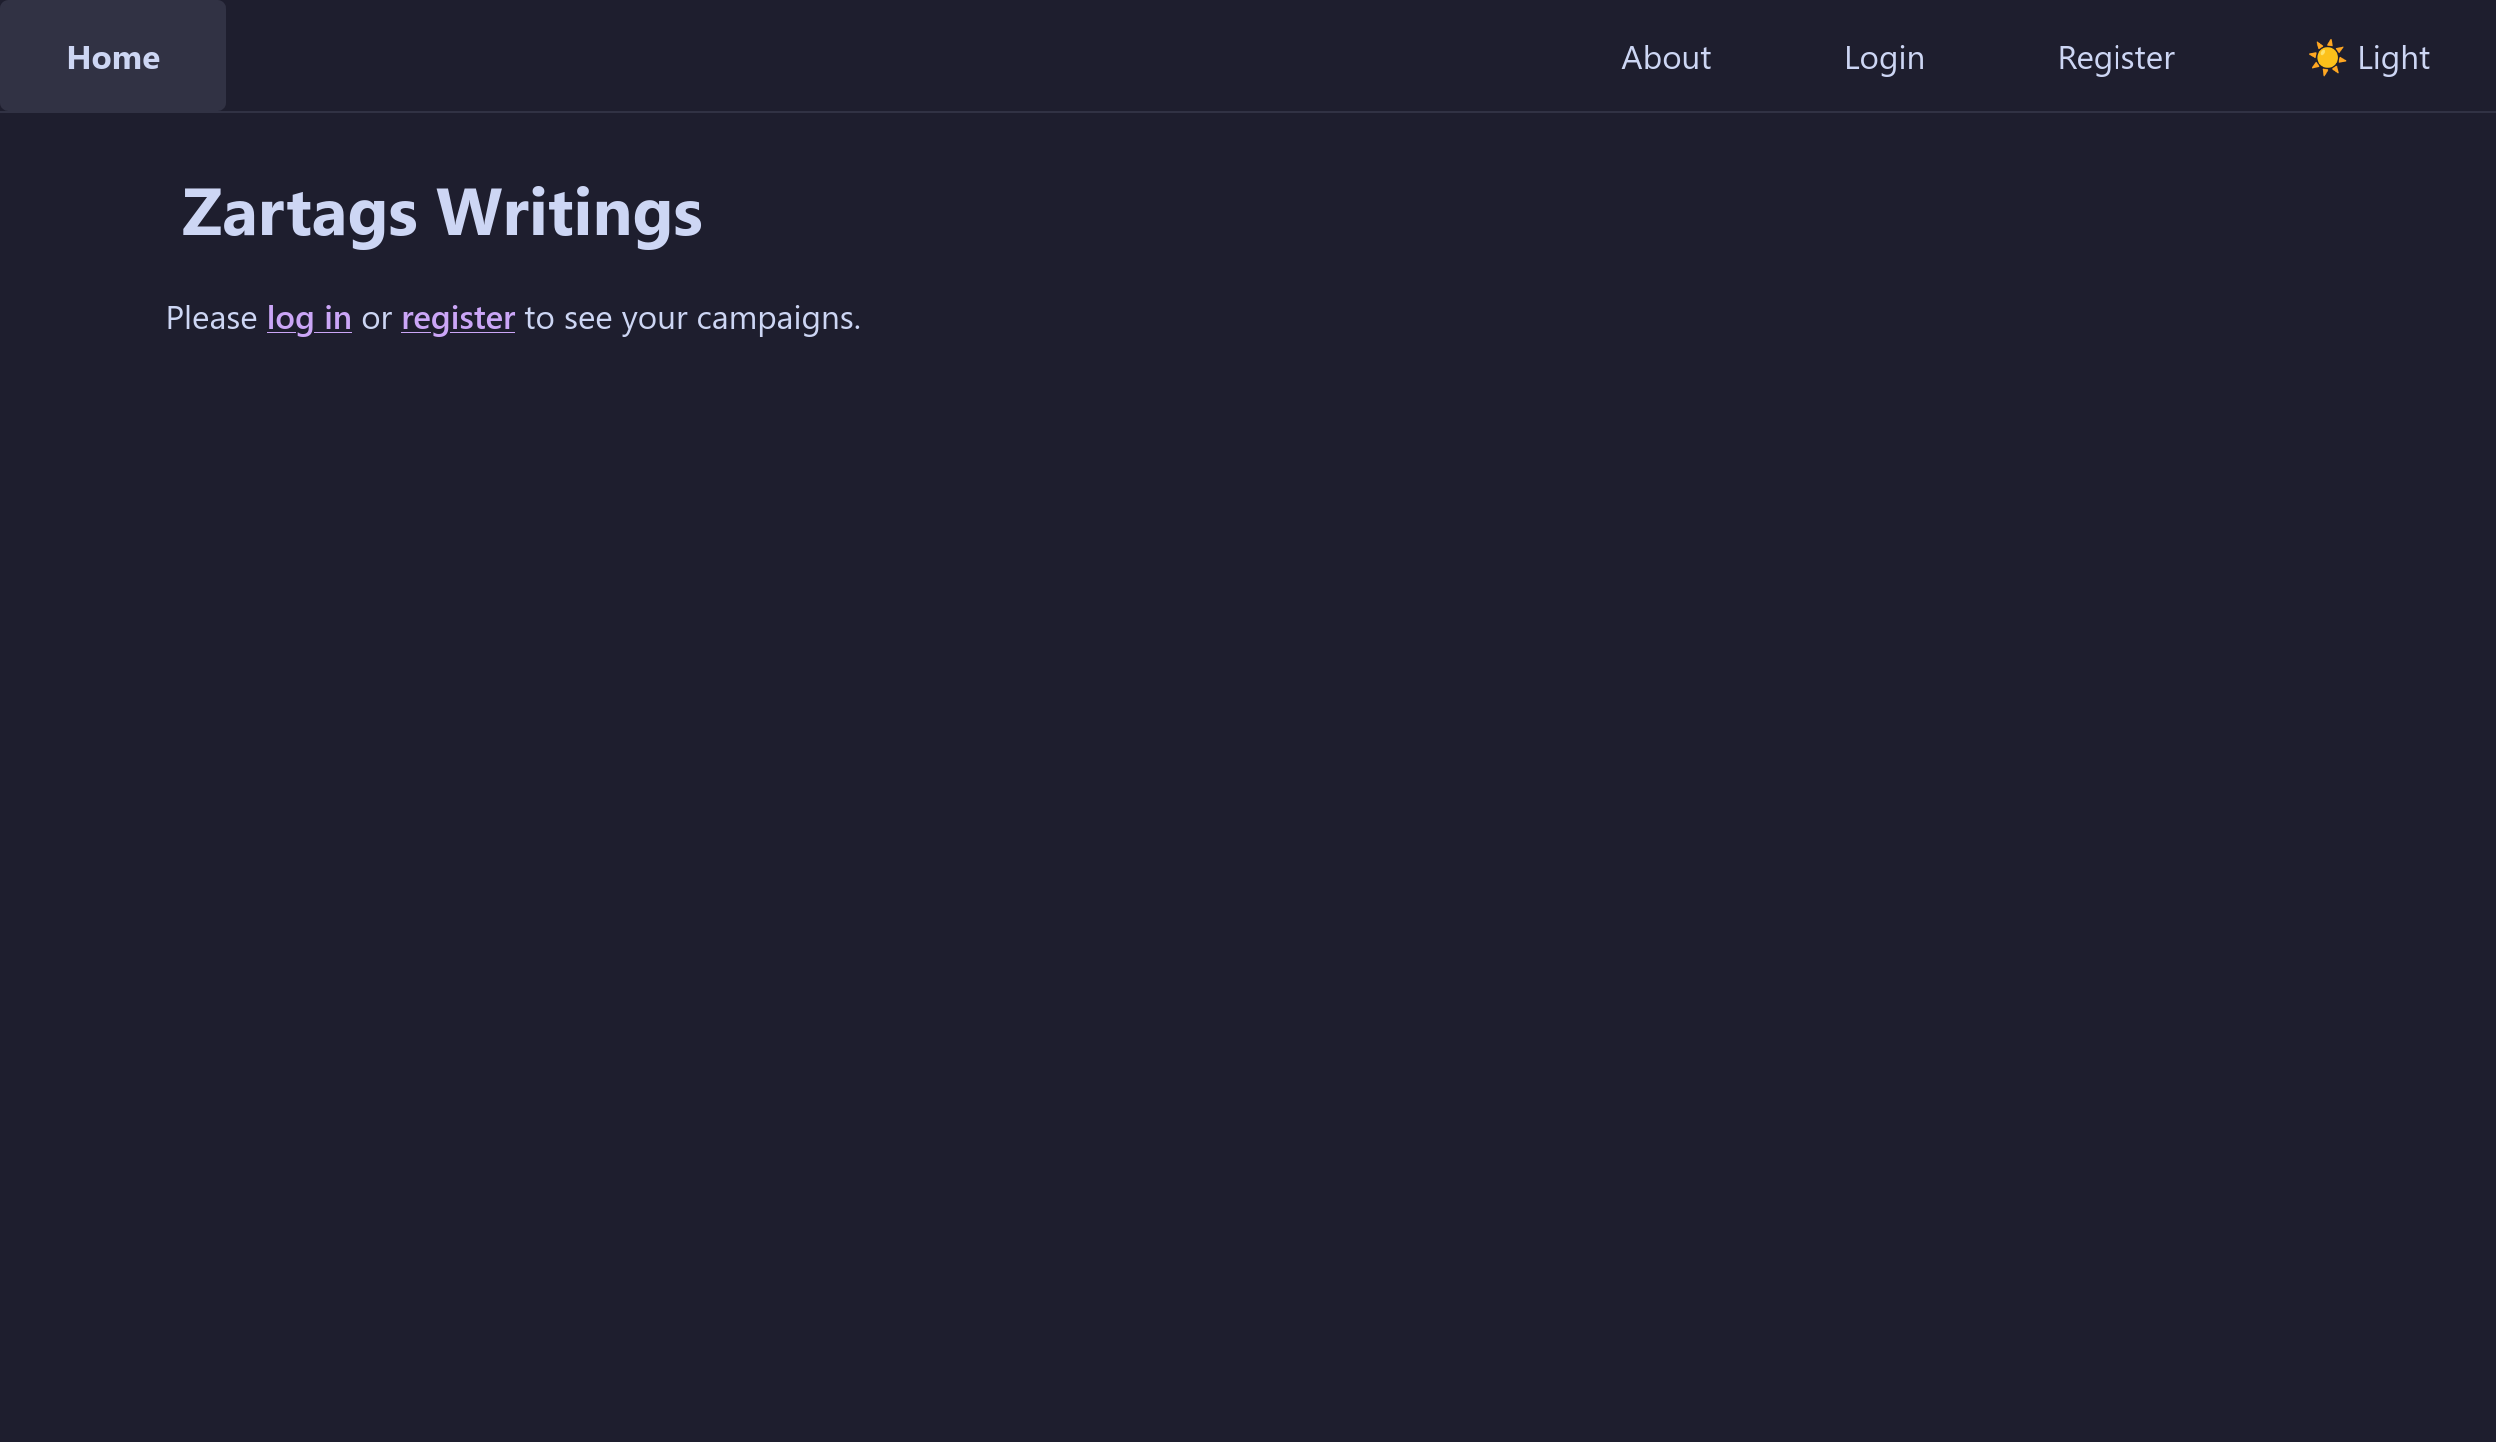
\includegraphics[width=0.92\textwidth]{media/Home_Default.png}
  \caption{Startseite ohne Login (Home Default)}
\end{figure}

\begin{figure}[H]
  \centering
  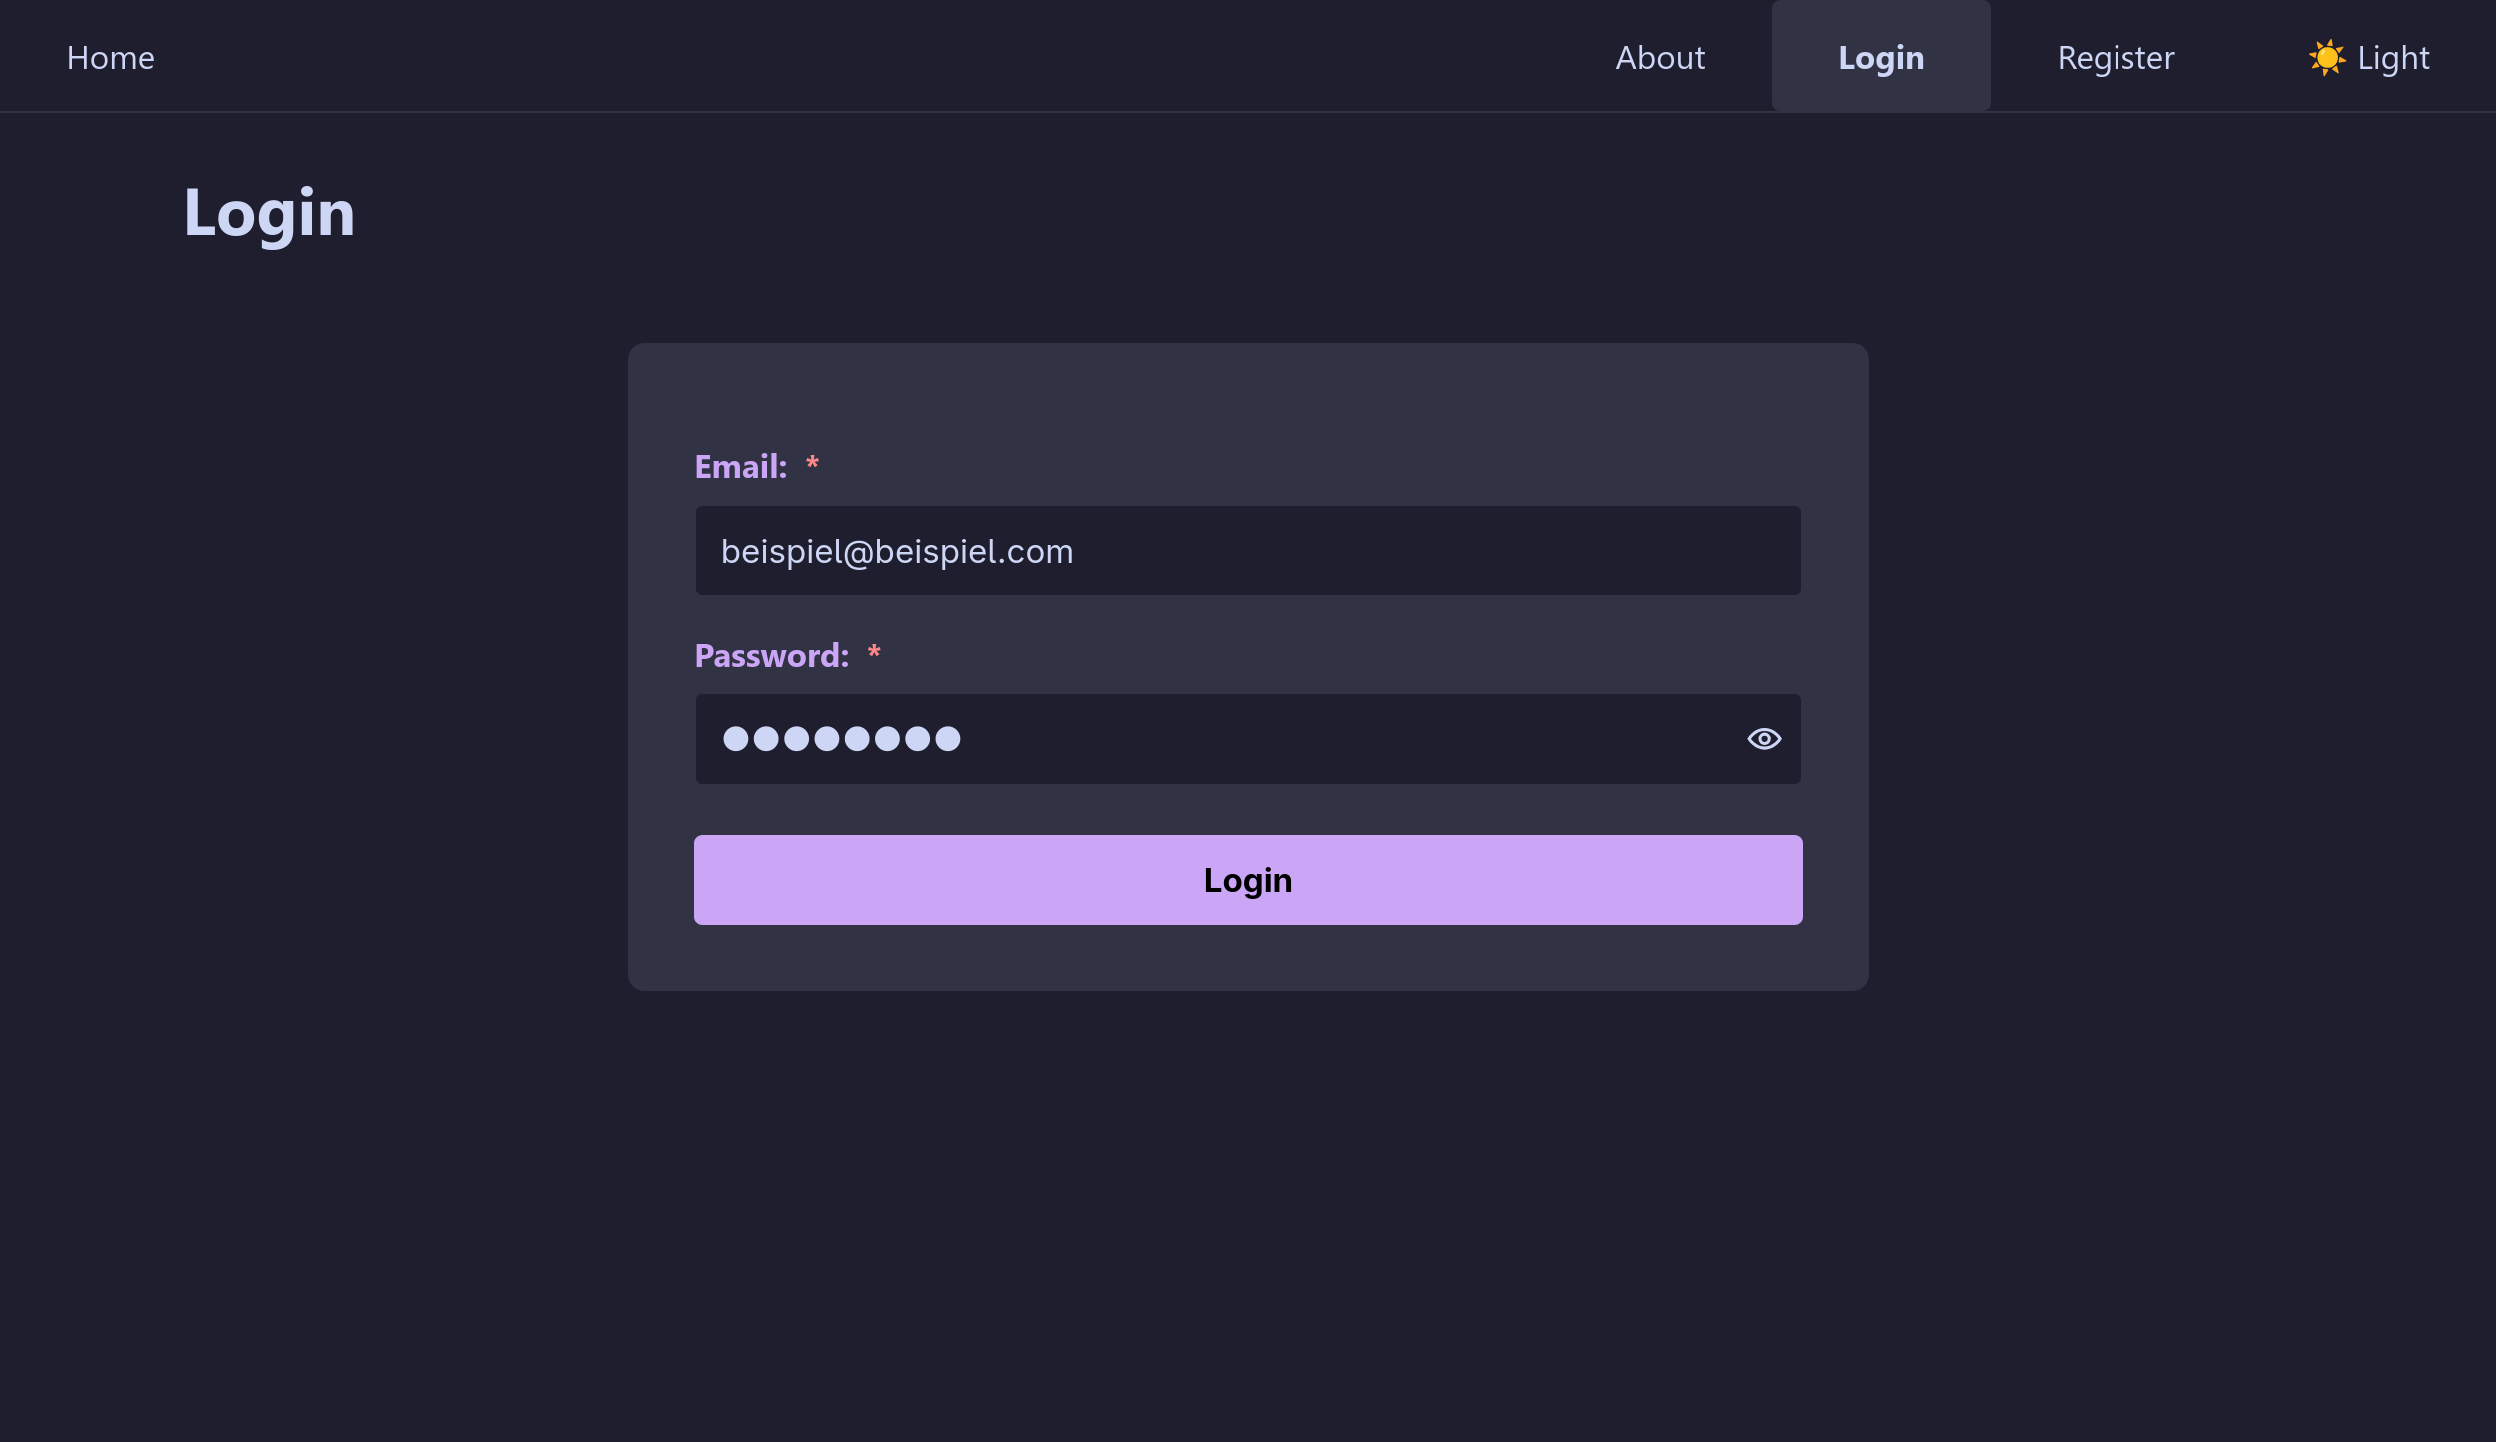
\includegraphics[width=0.92\textwidth]{media/Login_Page.png}
  \caption{Login-Seite}
\end{figure}

\begin{figure}[H]
  \centering
  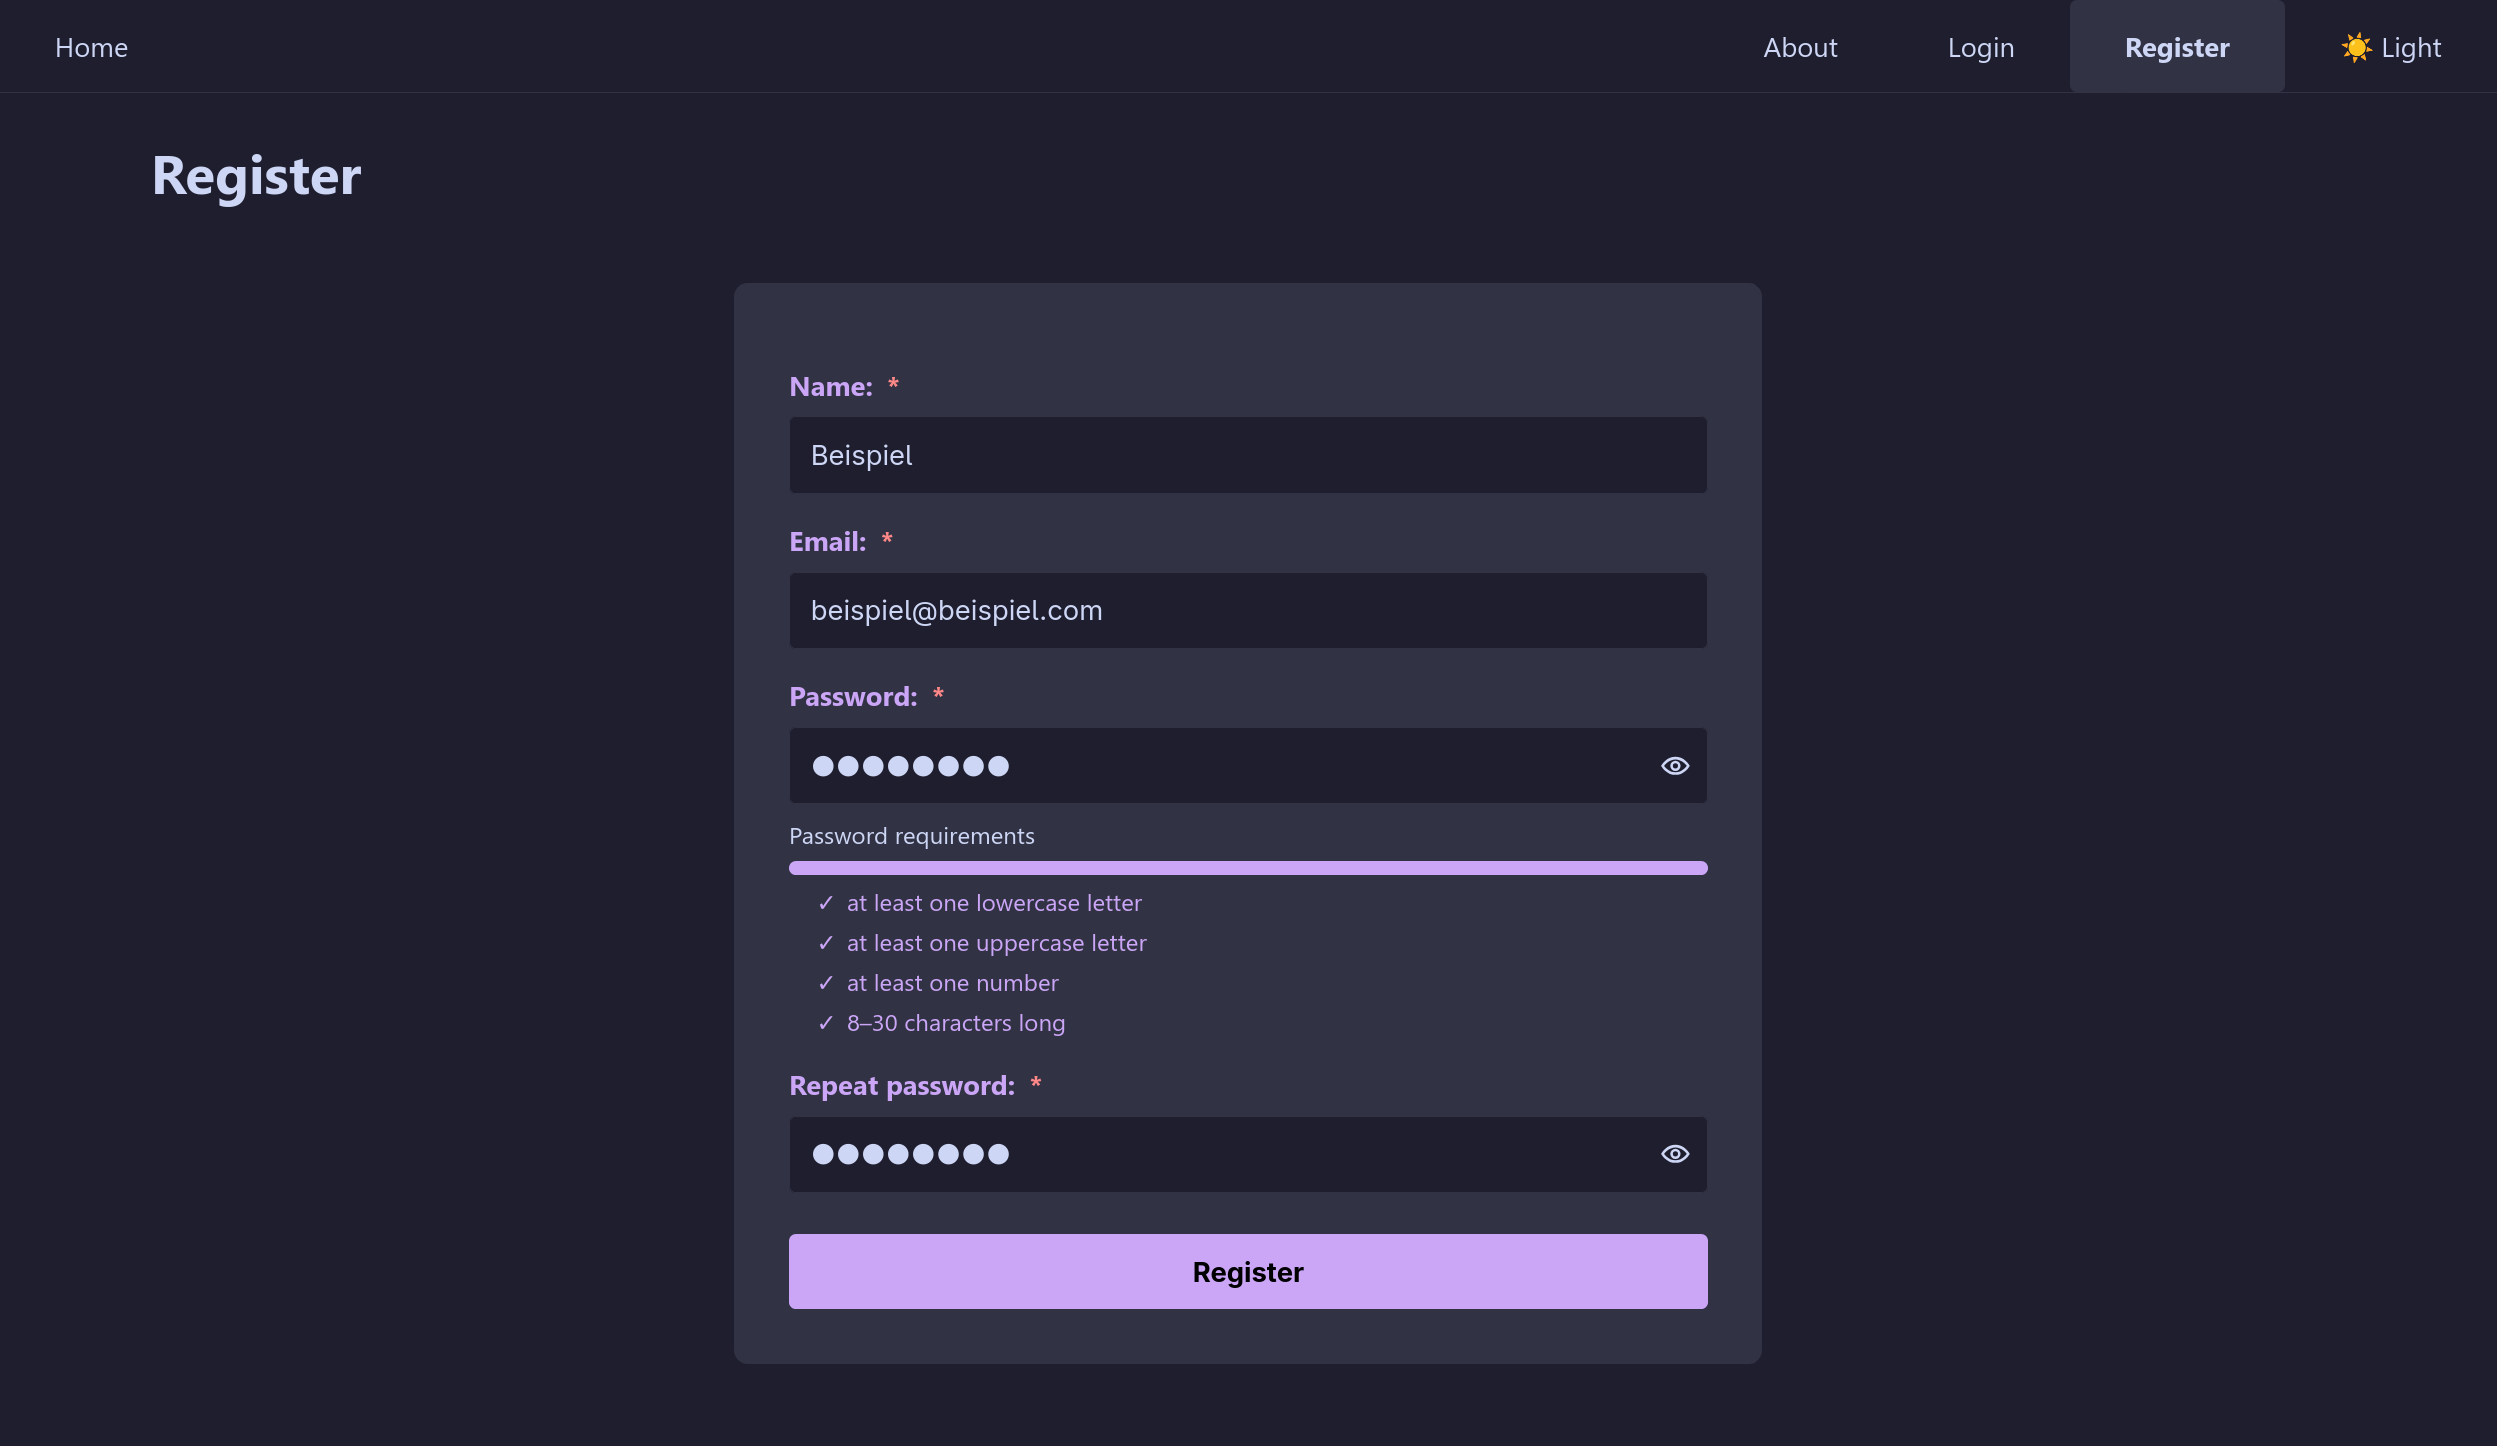
\includegraphics[width=0.92\textwidth]{media/Register_Page.png}
  \caption{Registrierungsseite}
\end{figure}

\begin{figure}[H]
  \centering
  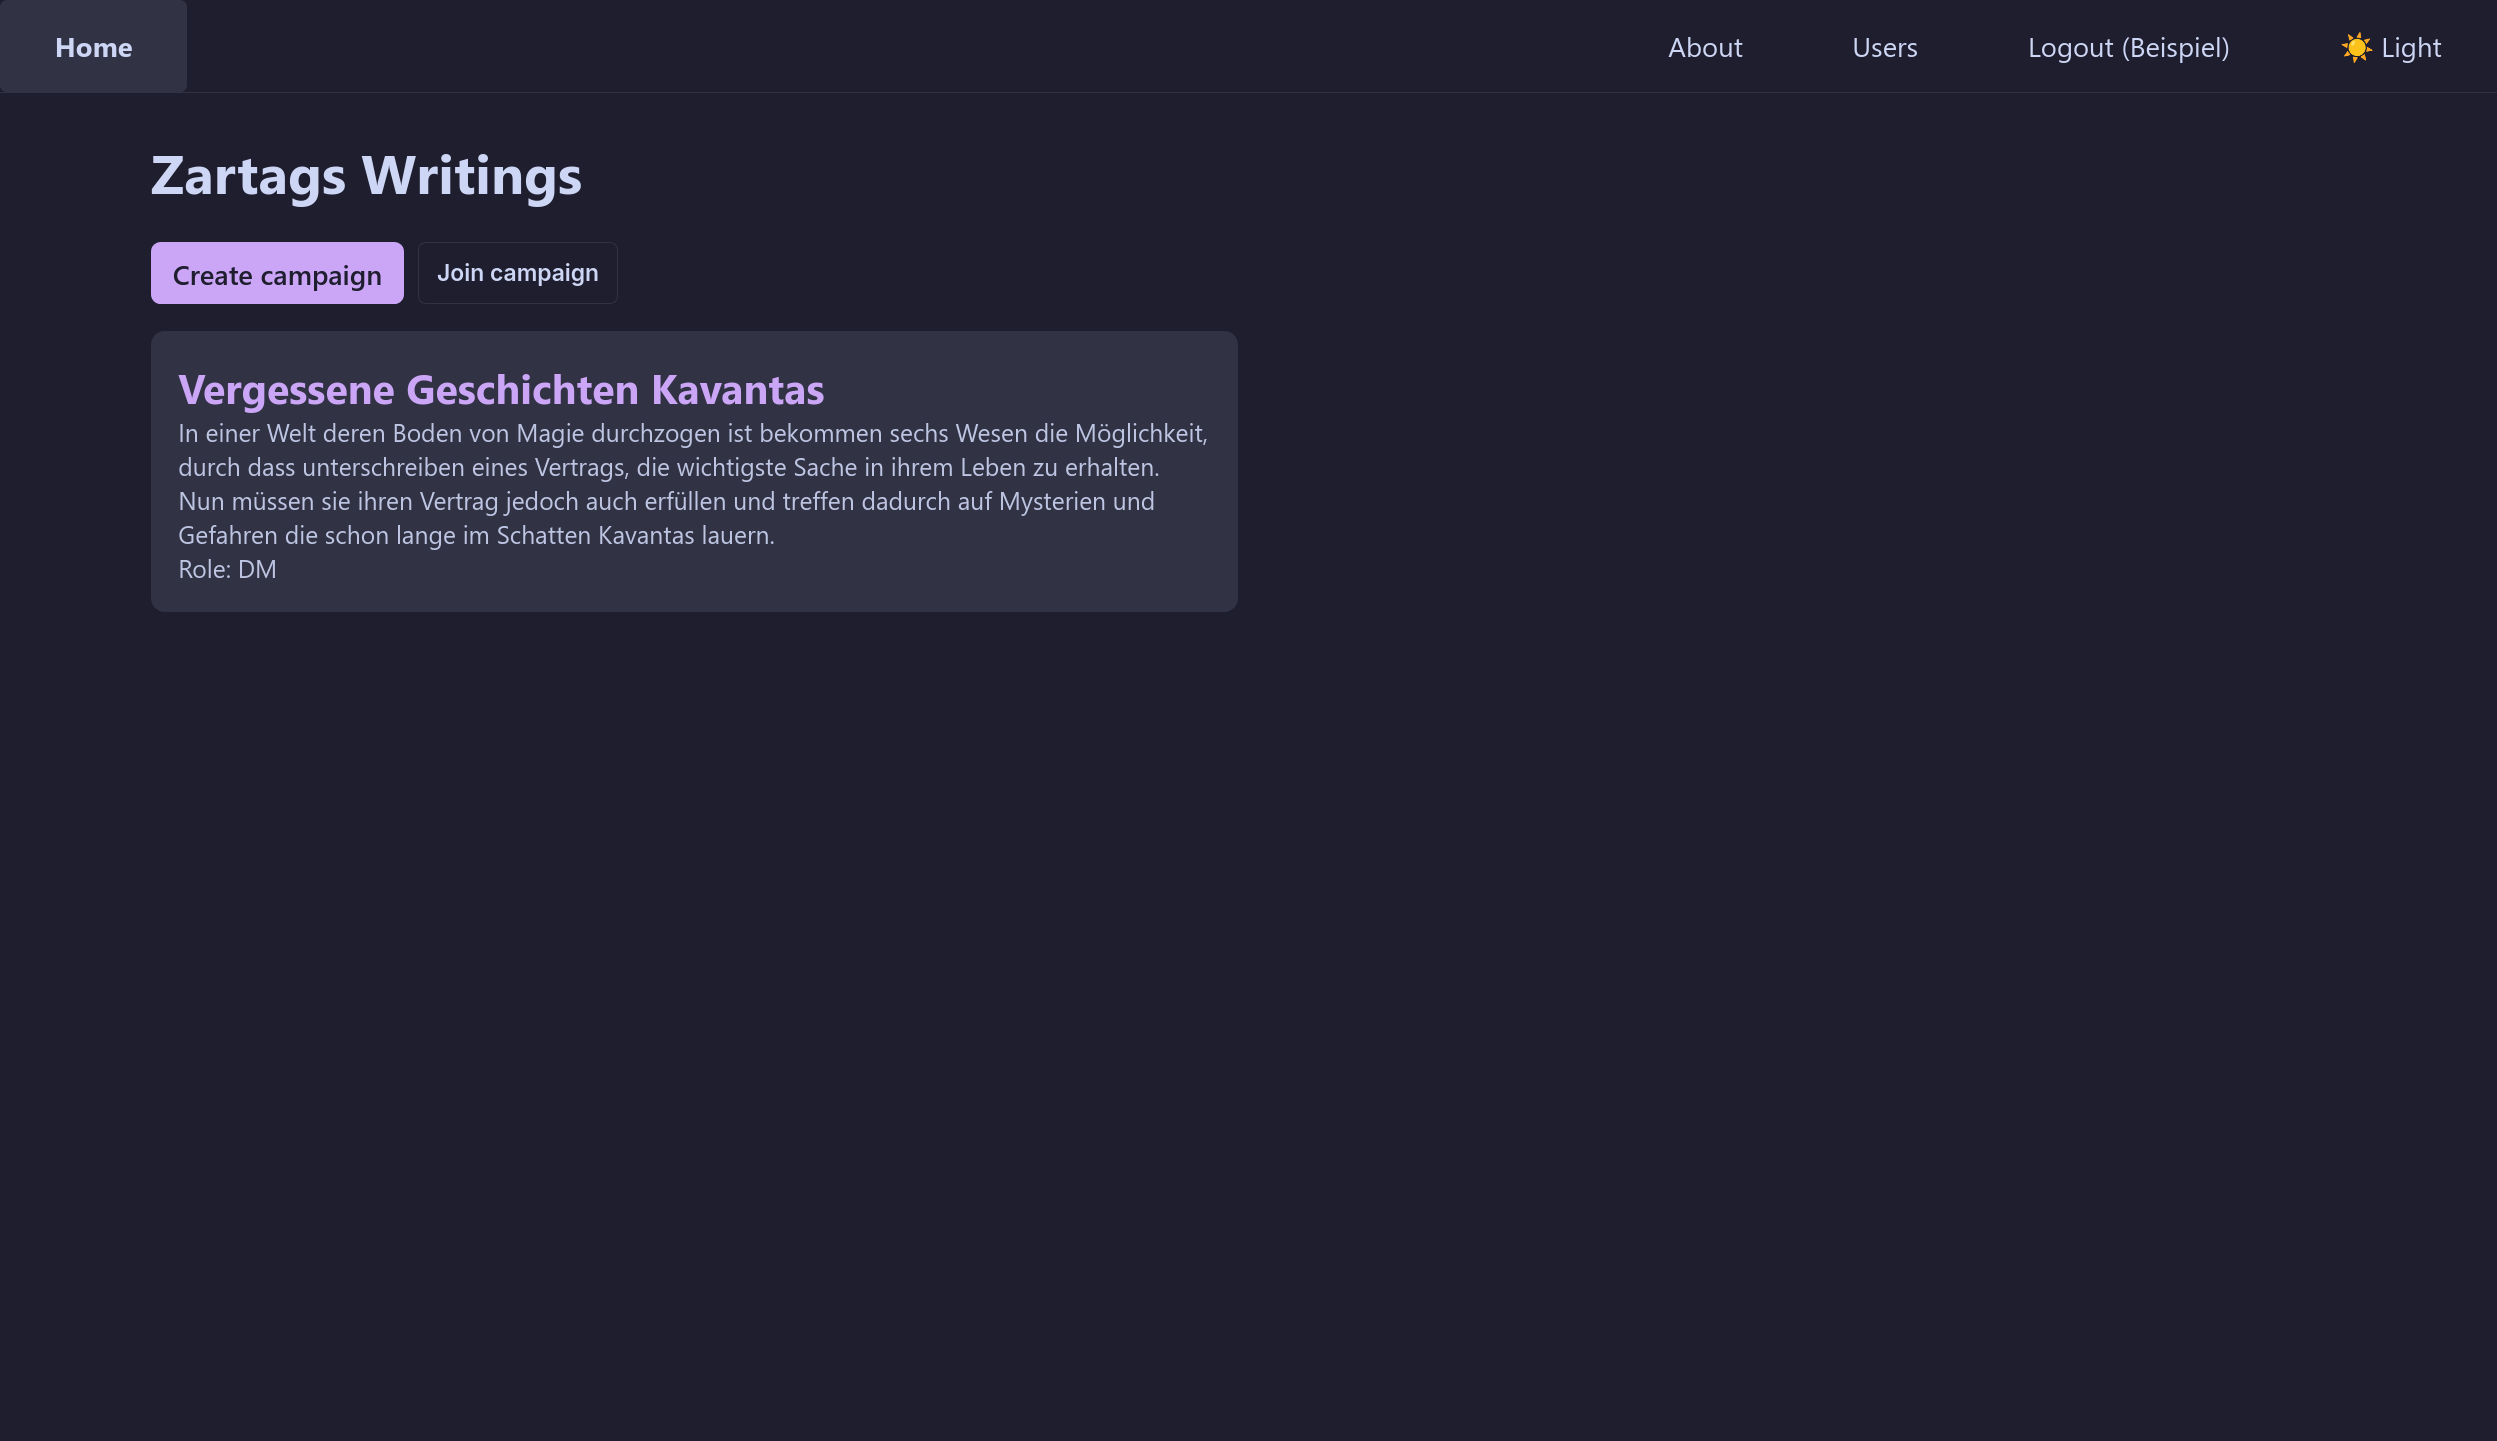
\includegraphics[width=0.92\textwidth]{media/Home_Logged_In.png}
  \caption{Startseite nach Login}
\end{figure}

\begin{figure}[H]
  \centering
  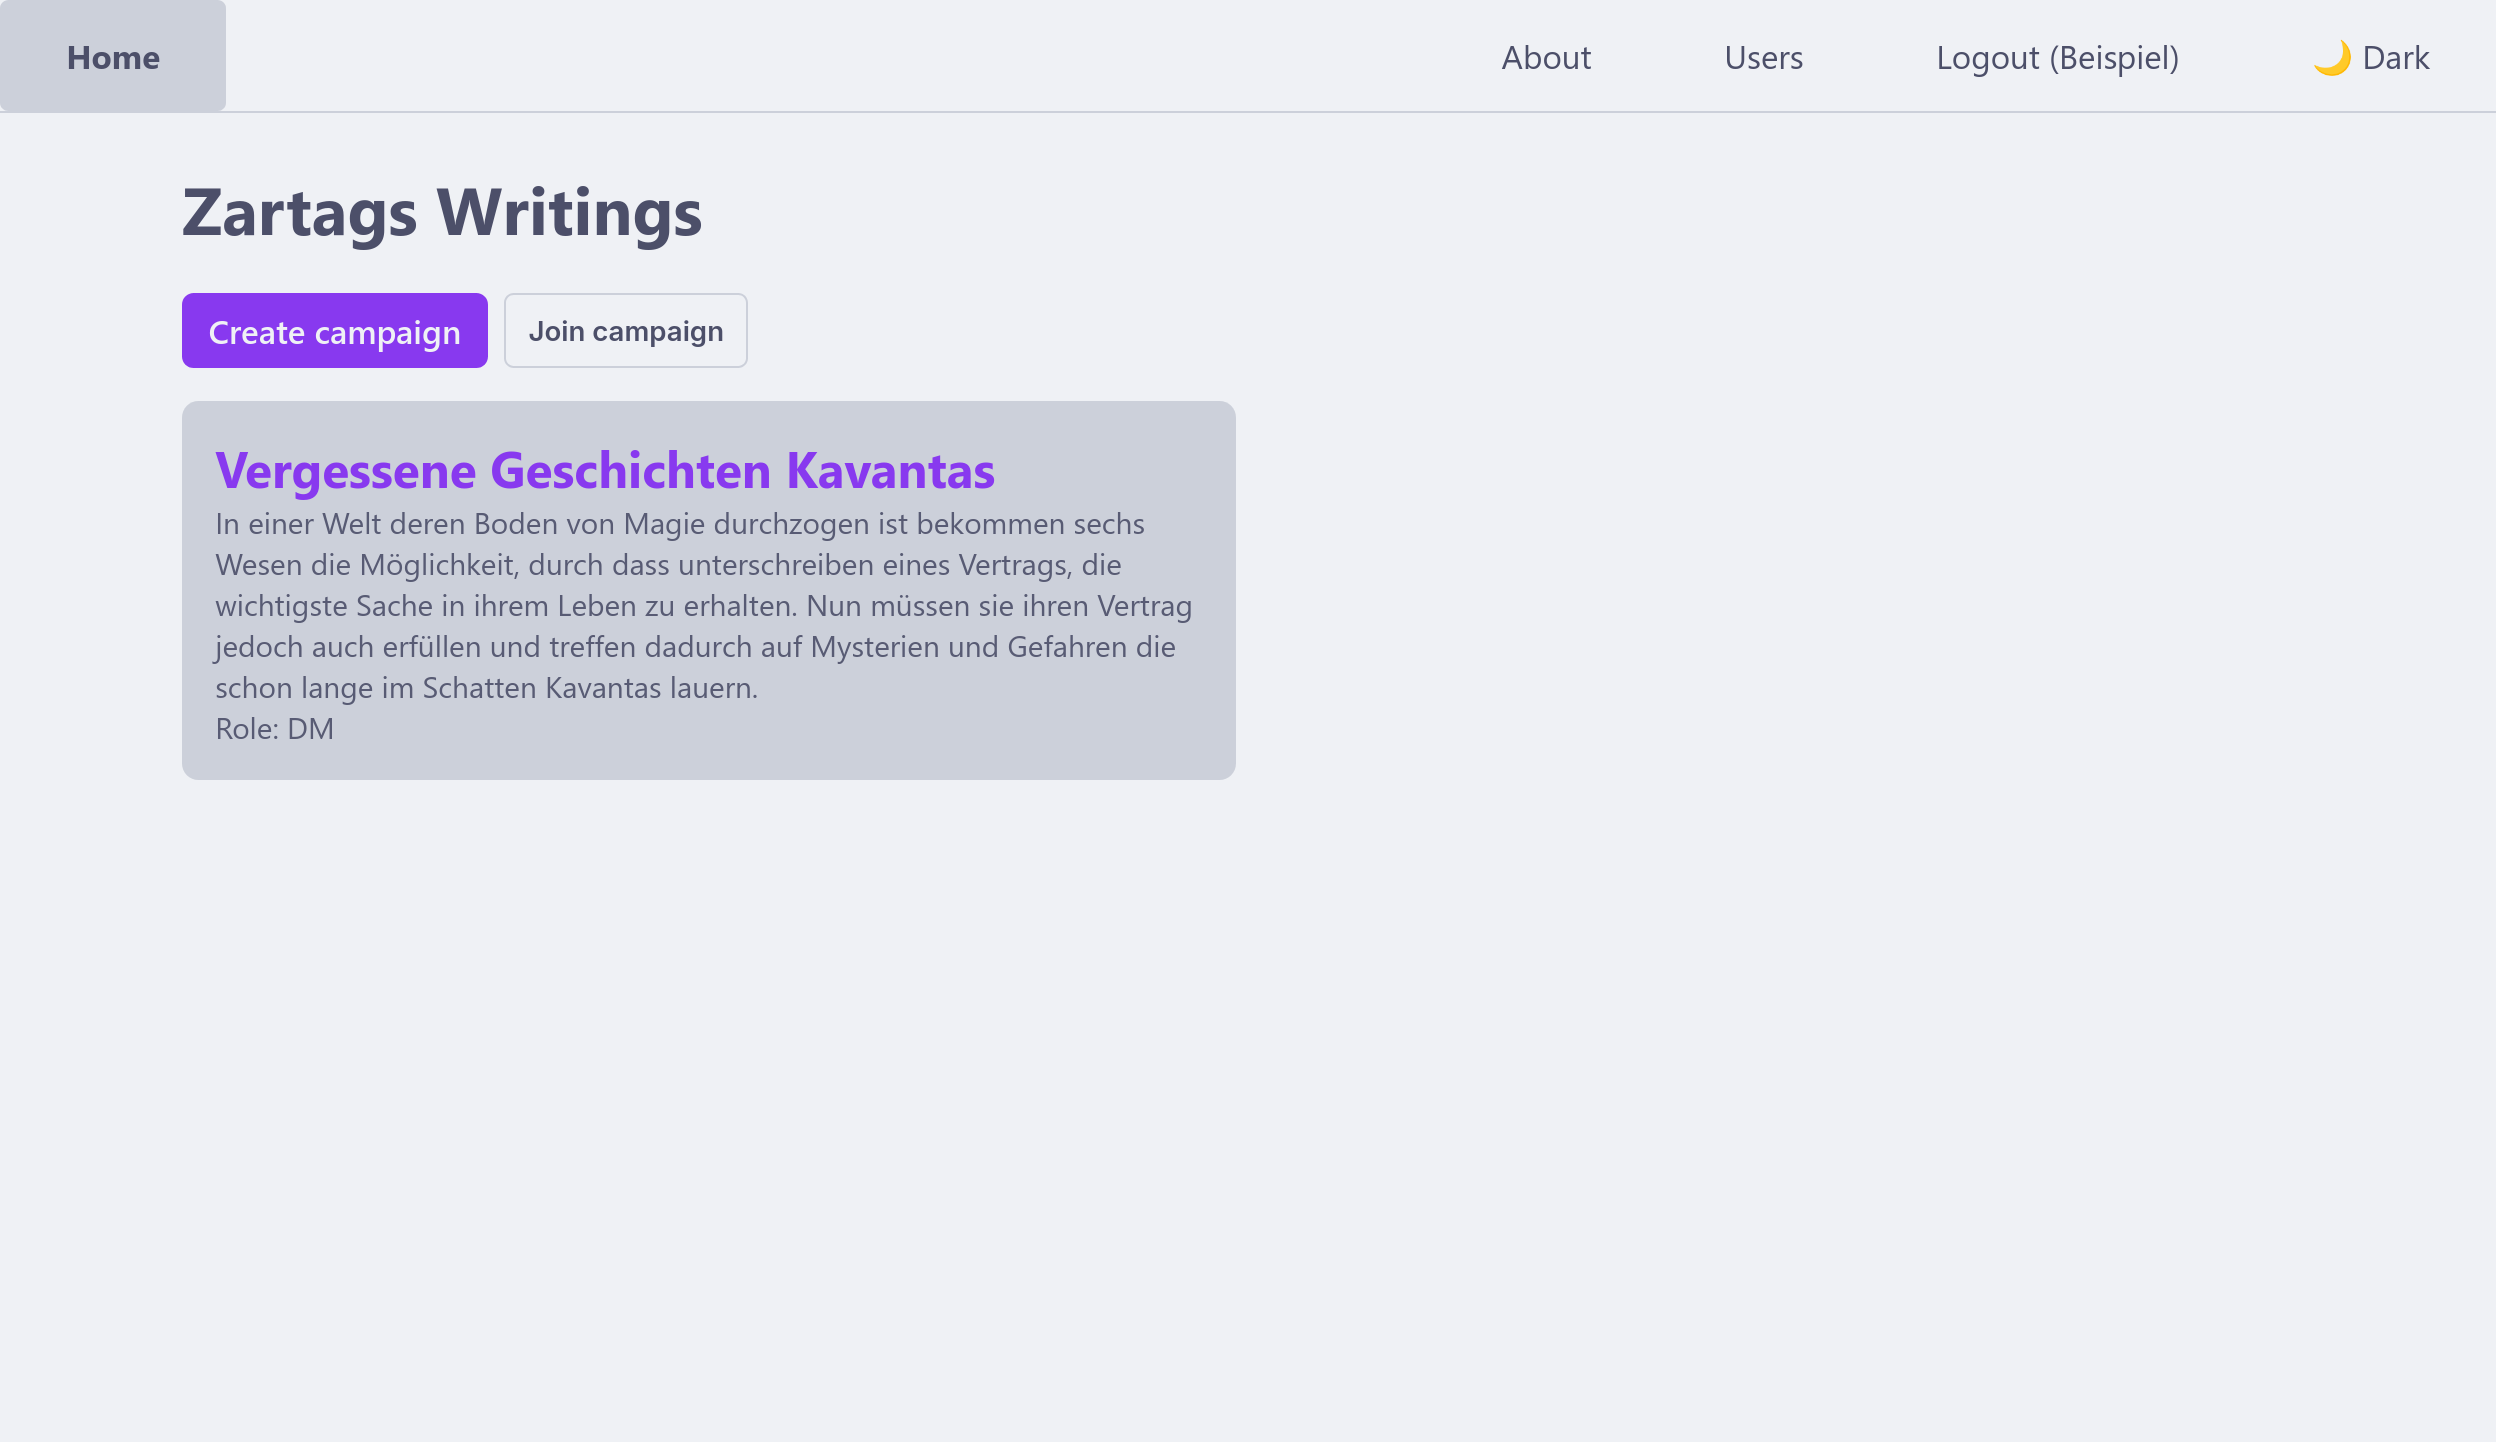
\includegraphics[width=0.92\textwidth]{media/LightMode_Home_Logged_In.png}
  \caption{Startseite nach Login im Light Mode}
\end{figure}

\begin{figure}[H]
  \centering
  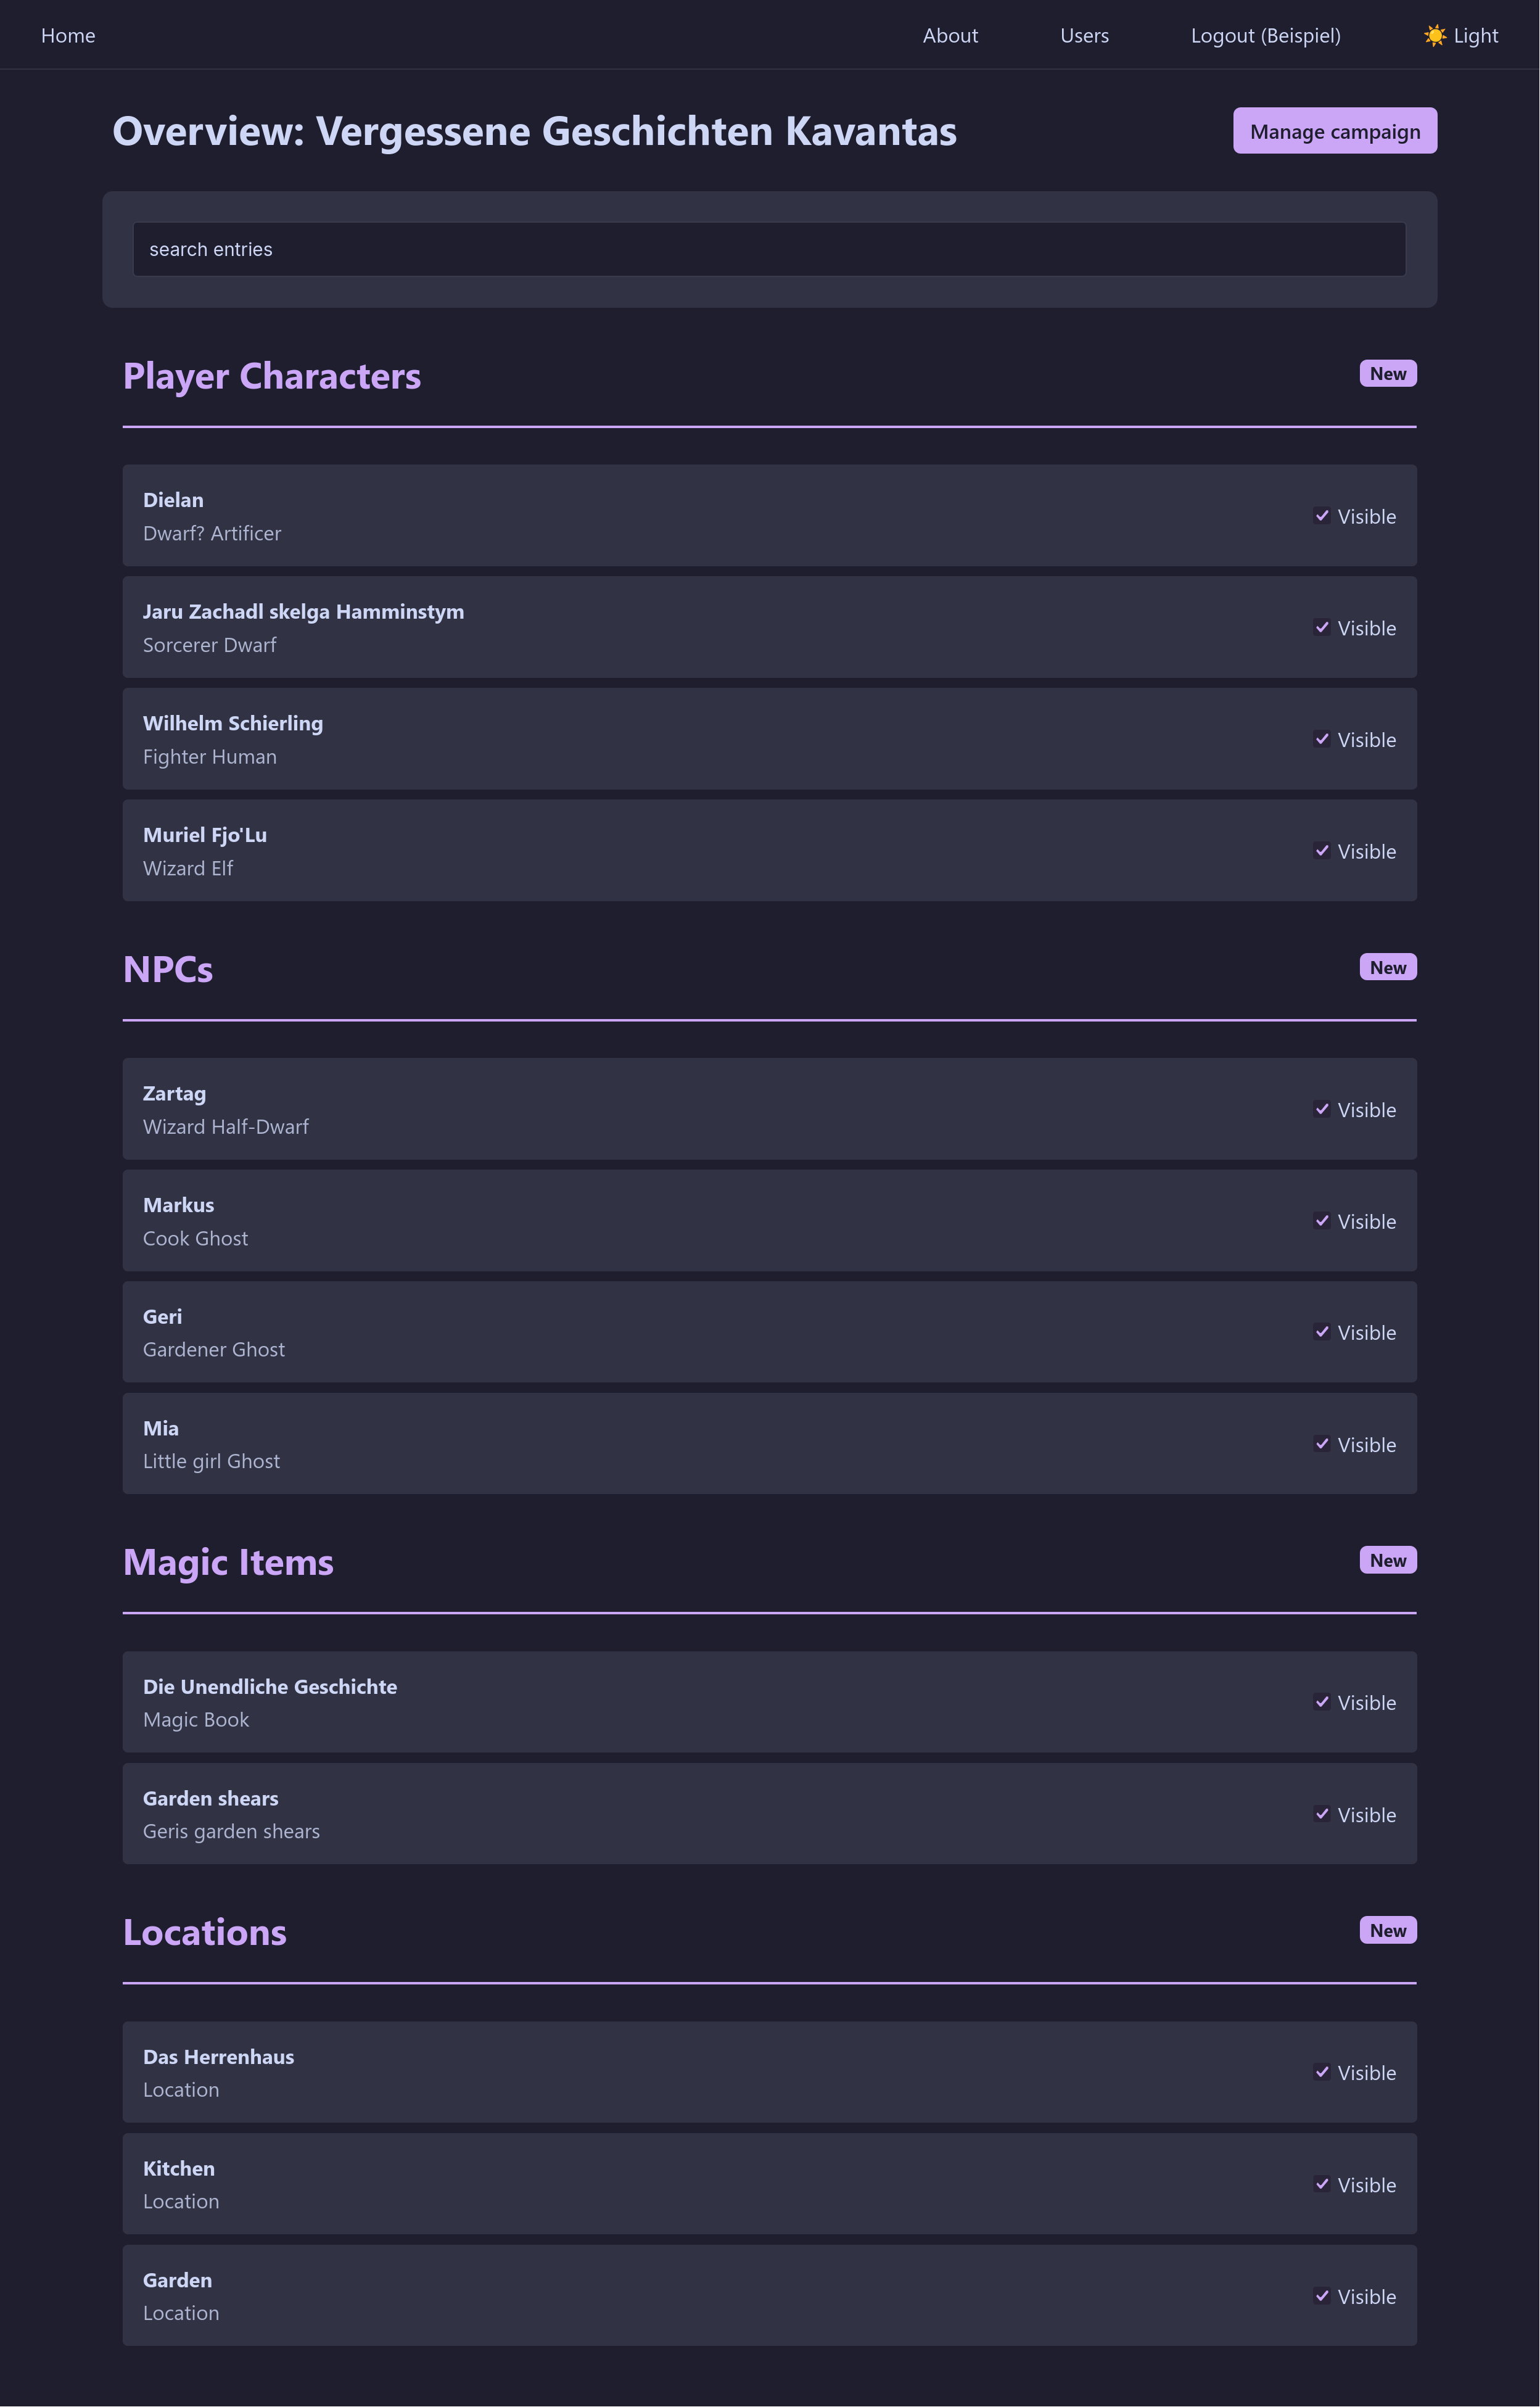
\includegraphics[width=0.92\textwidth]{media/Overview.png}
  \caption{Campaign-Übersicht mit Kategorien}
\end{figure}

\begin{figure}[H]
  \centering
  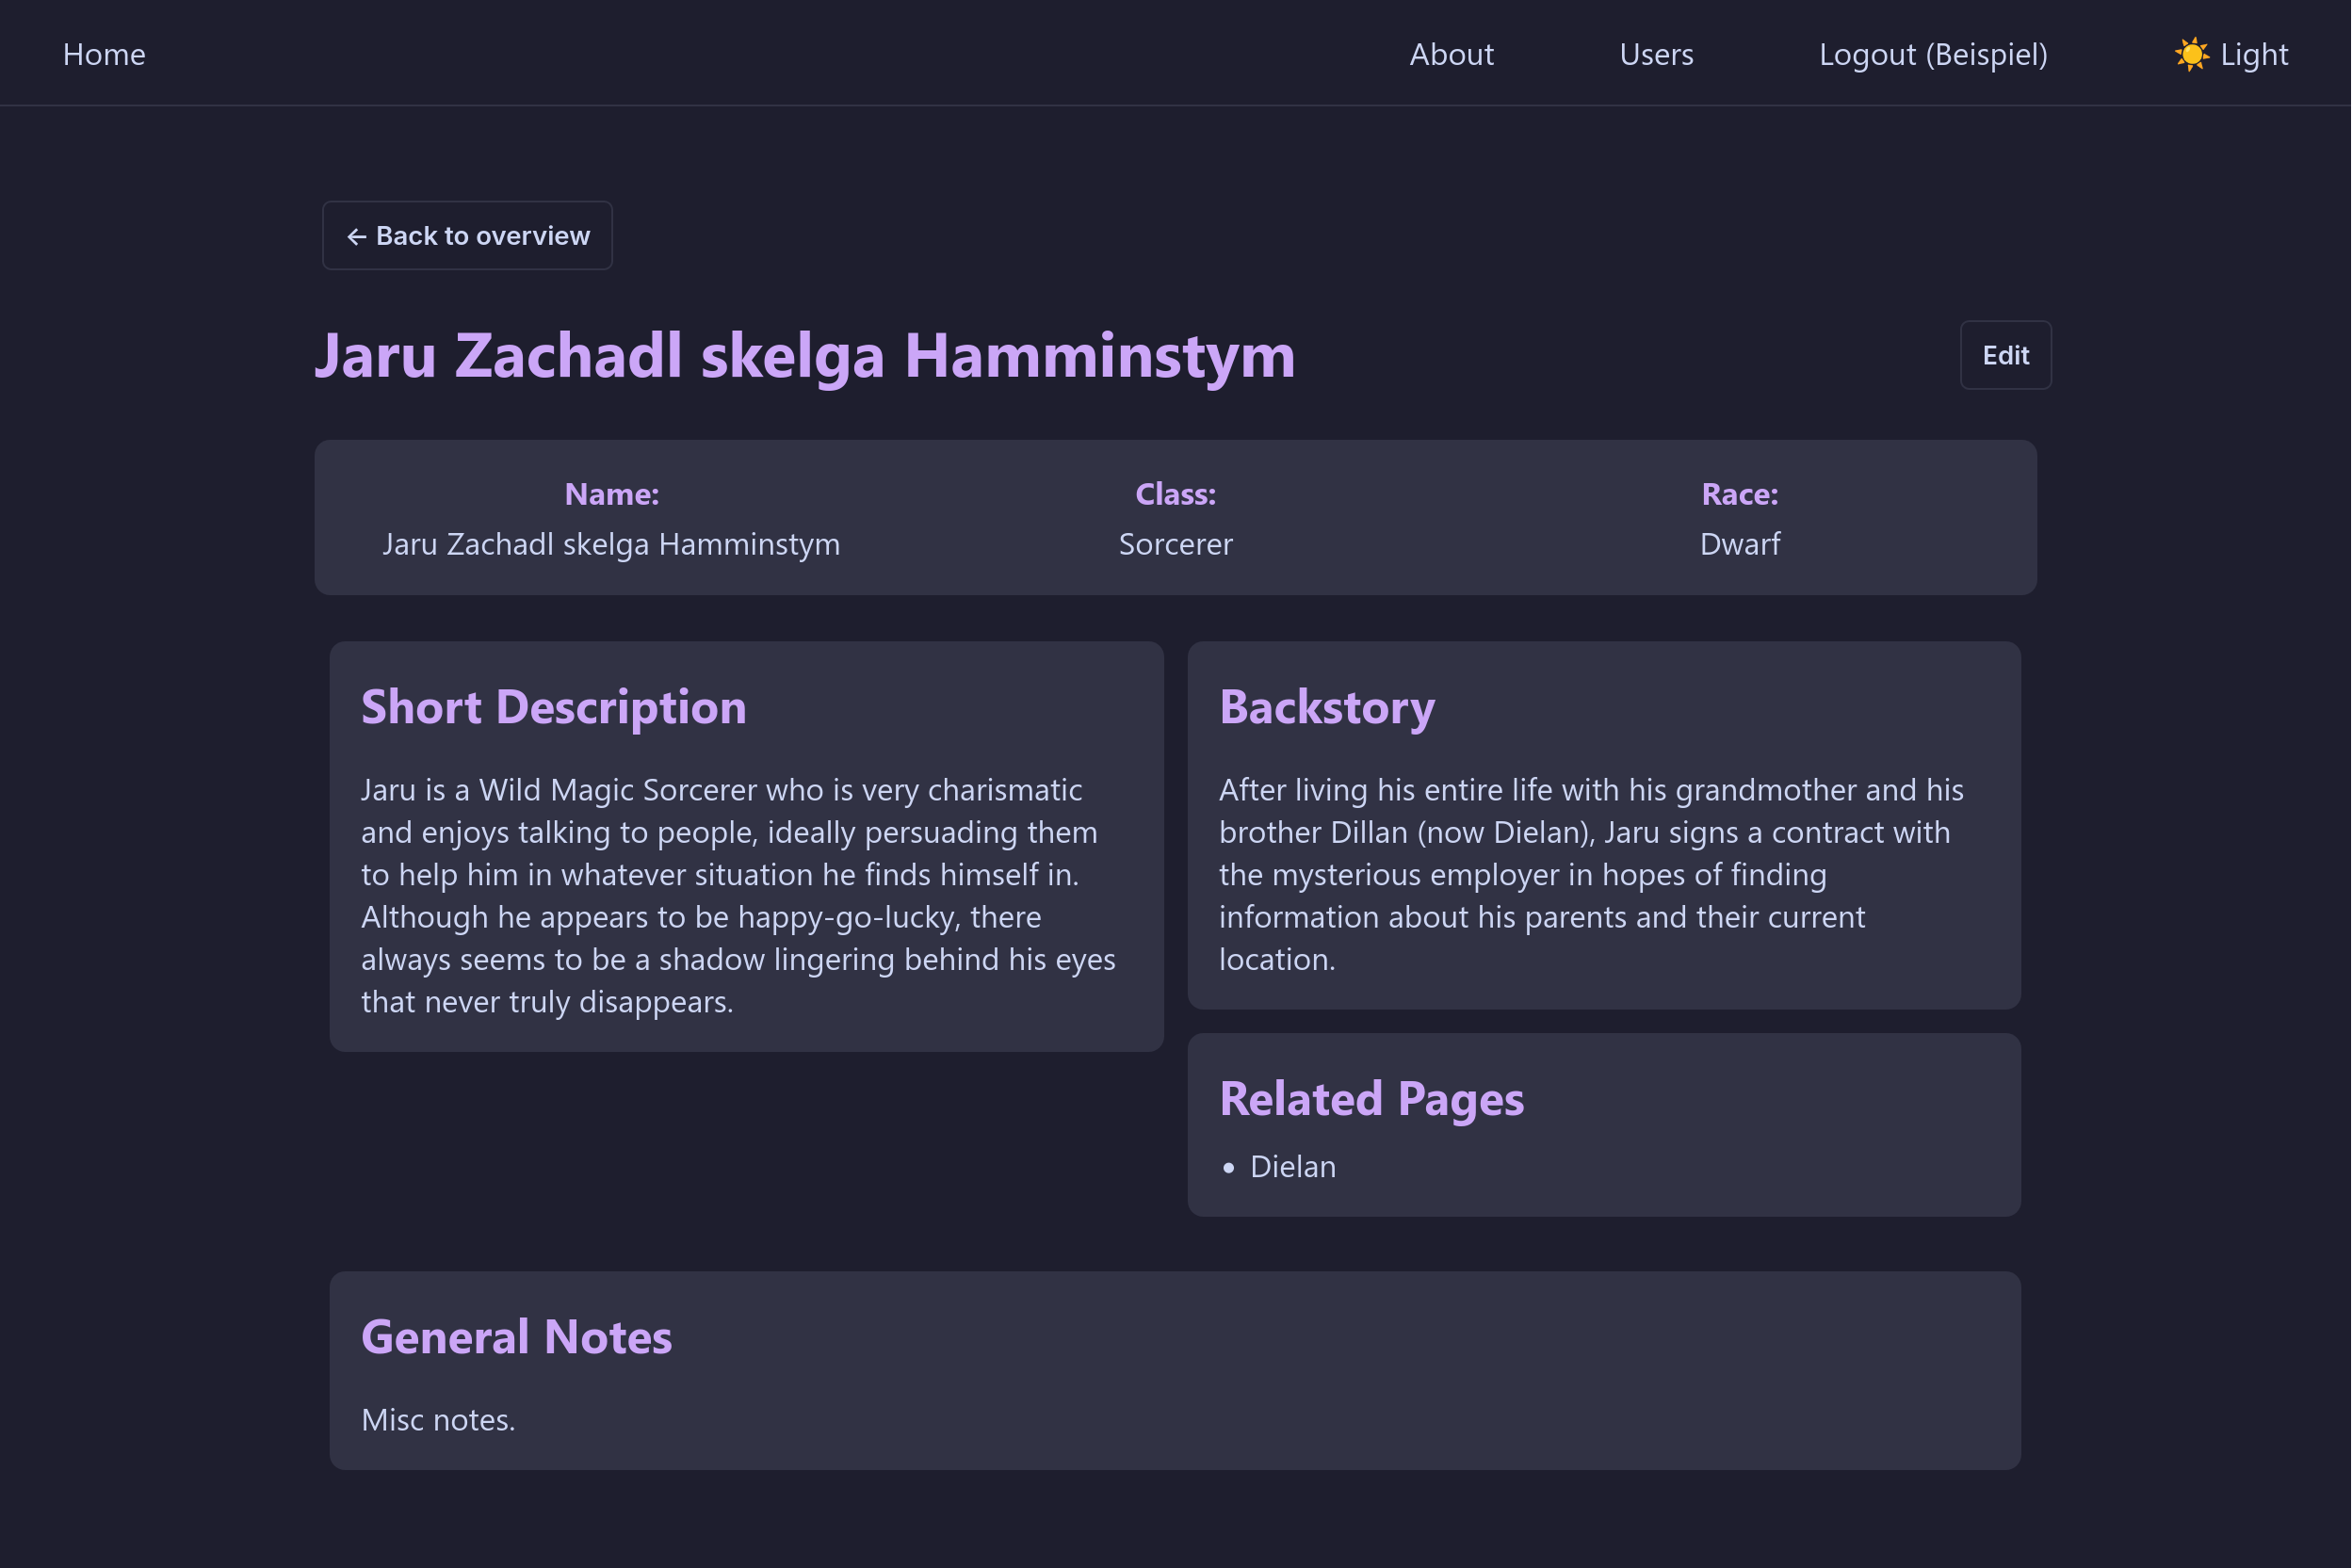
\includegraphics[width=0.92\textwidth]{media/PC.png}
  \caption{Entity-Detailansicht: Player Character}
\end{figure}

\begin{figure}[H]
  \centering
  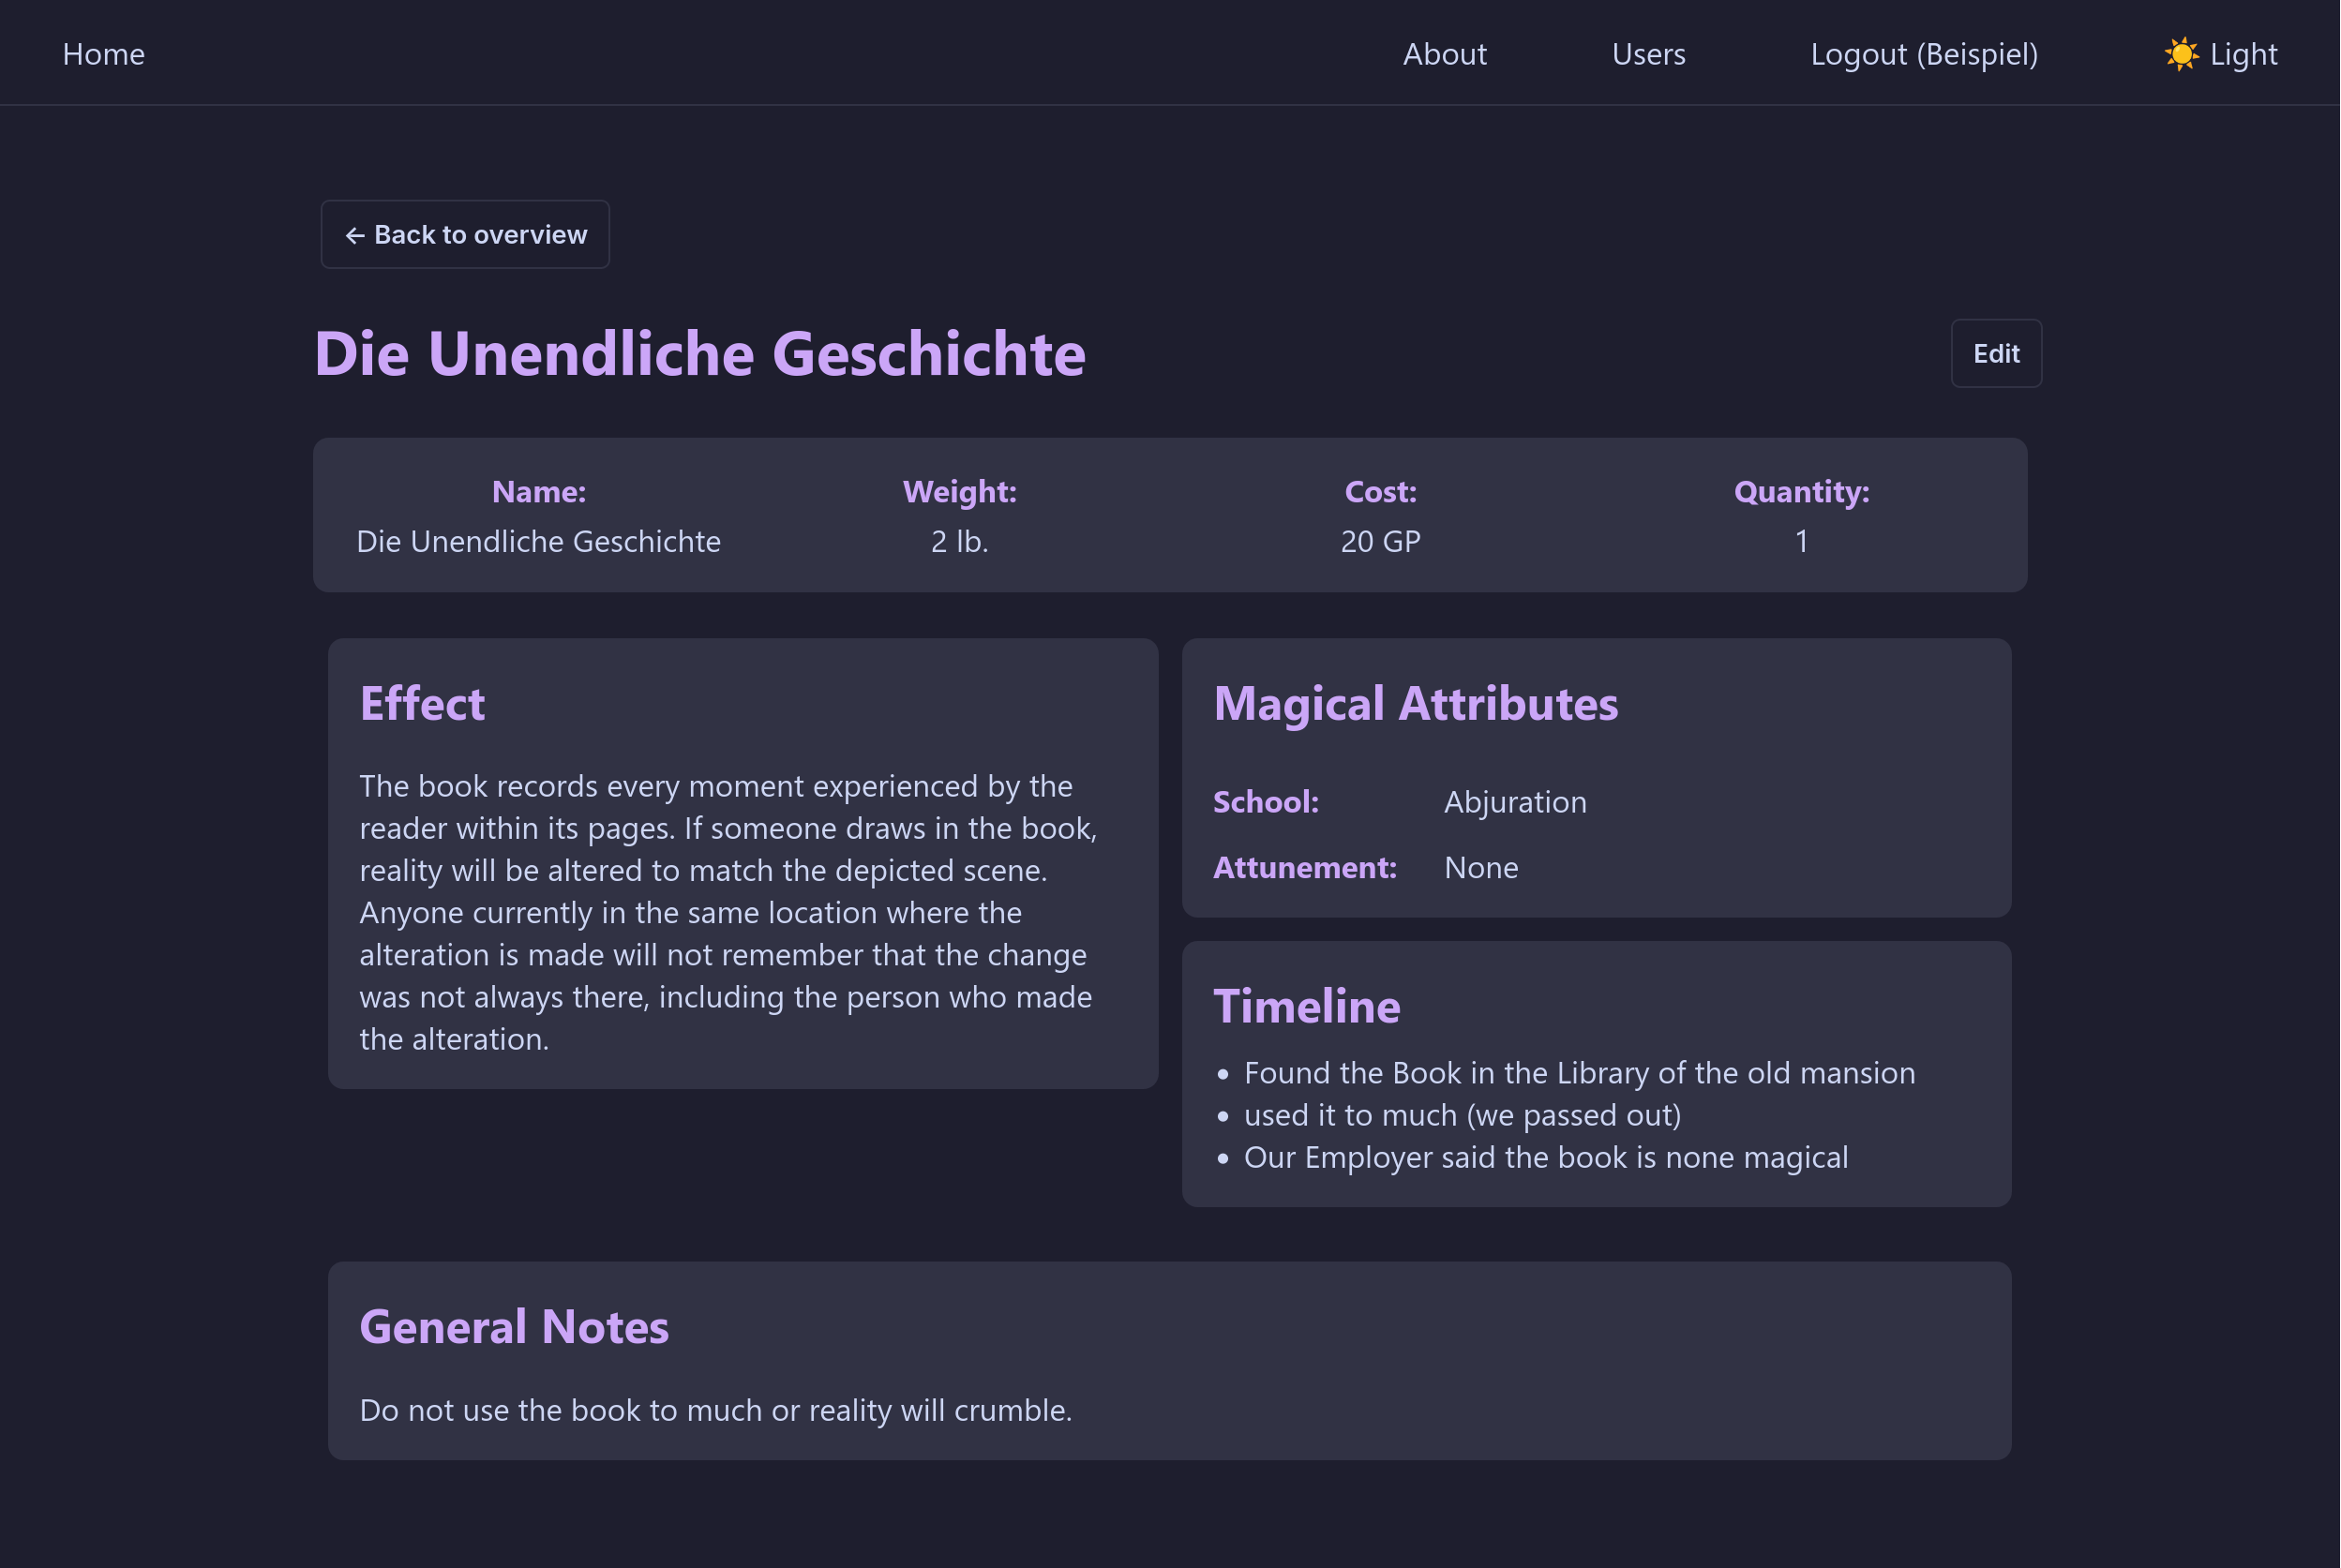
\includegraphics[width=0.92\textwidth]{media/Magic_Item.png}
  \caption{Entity-Detailansicht: Magic Item}
\end{figure}

\begin{figure}[H]
  \centering
  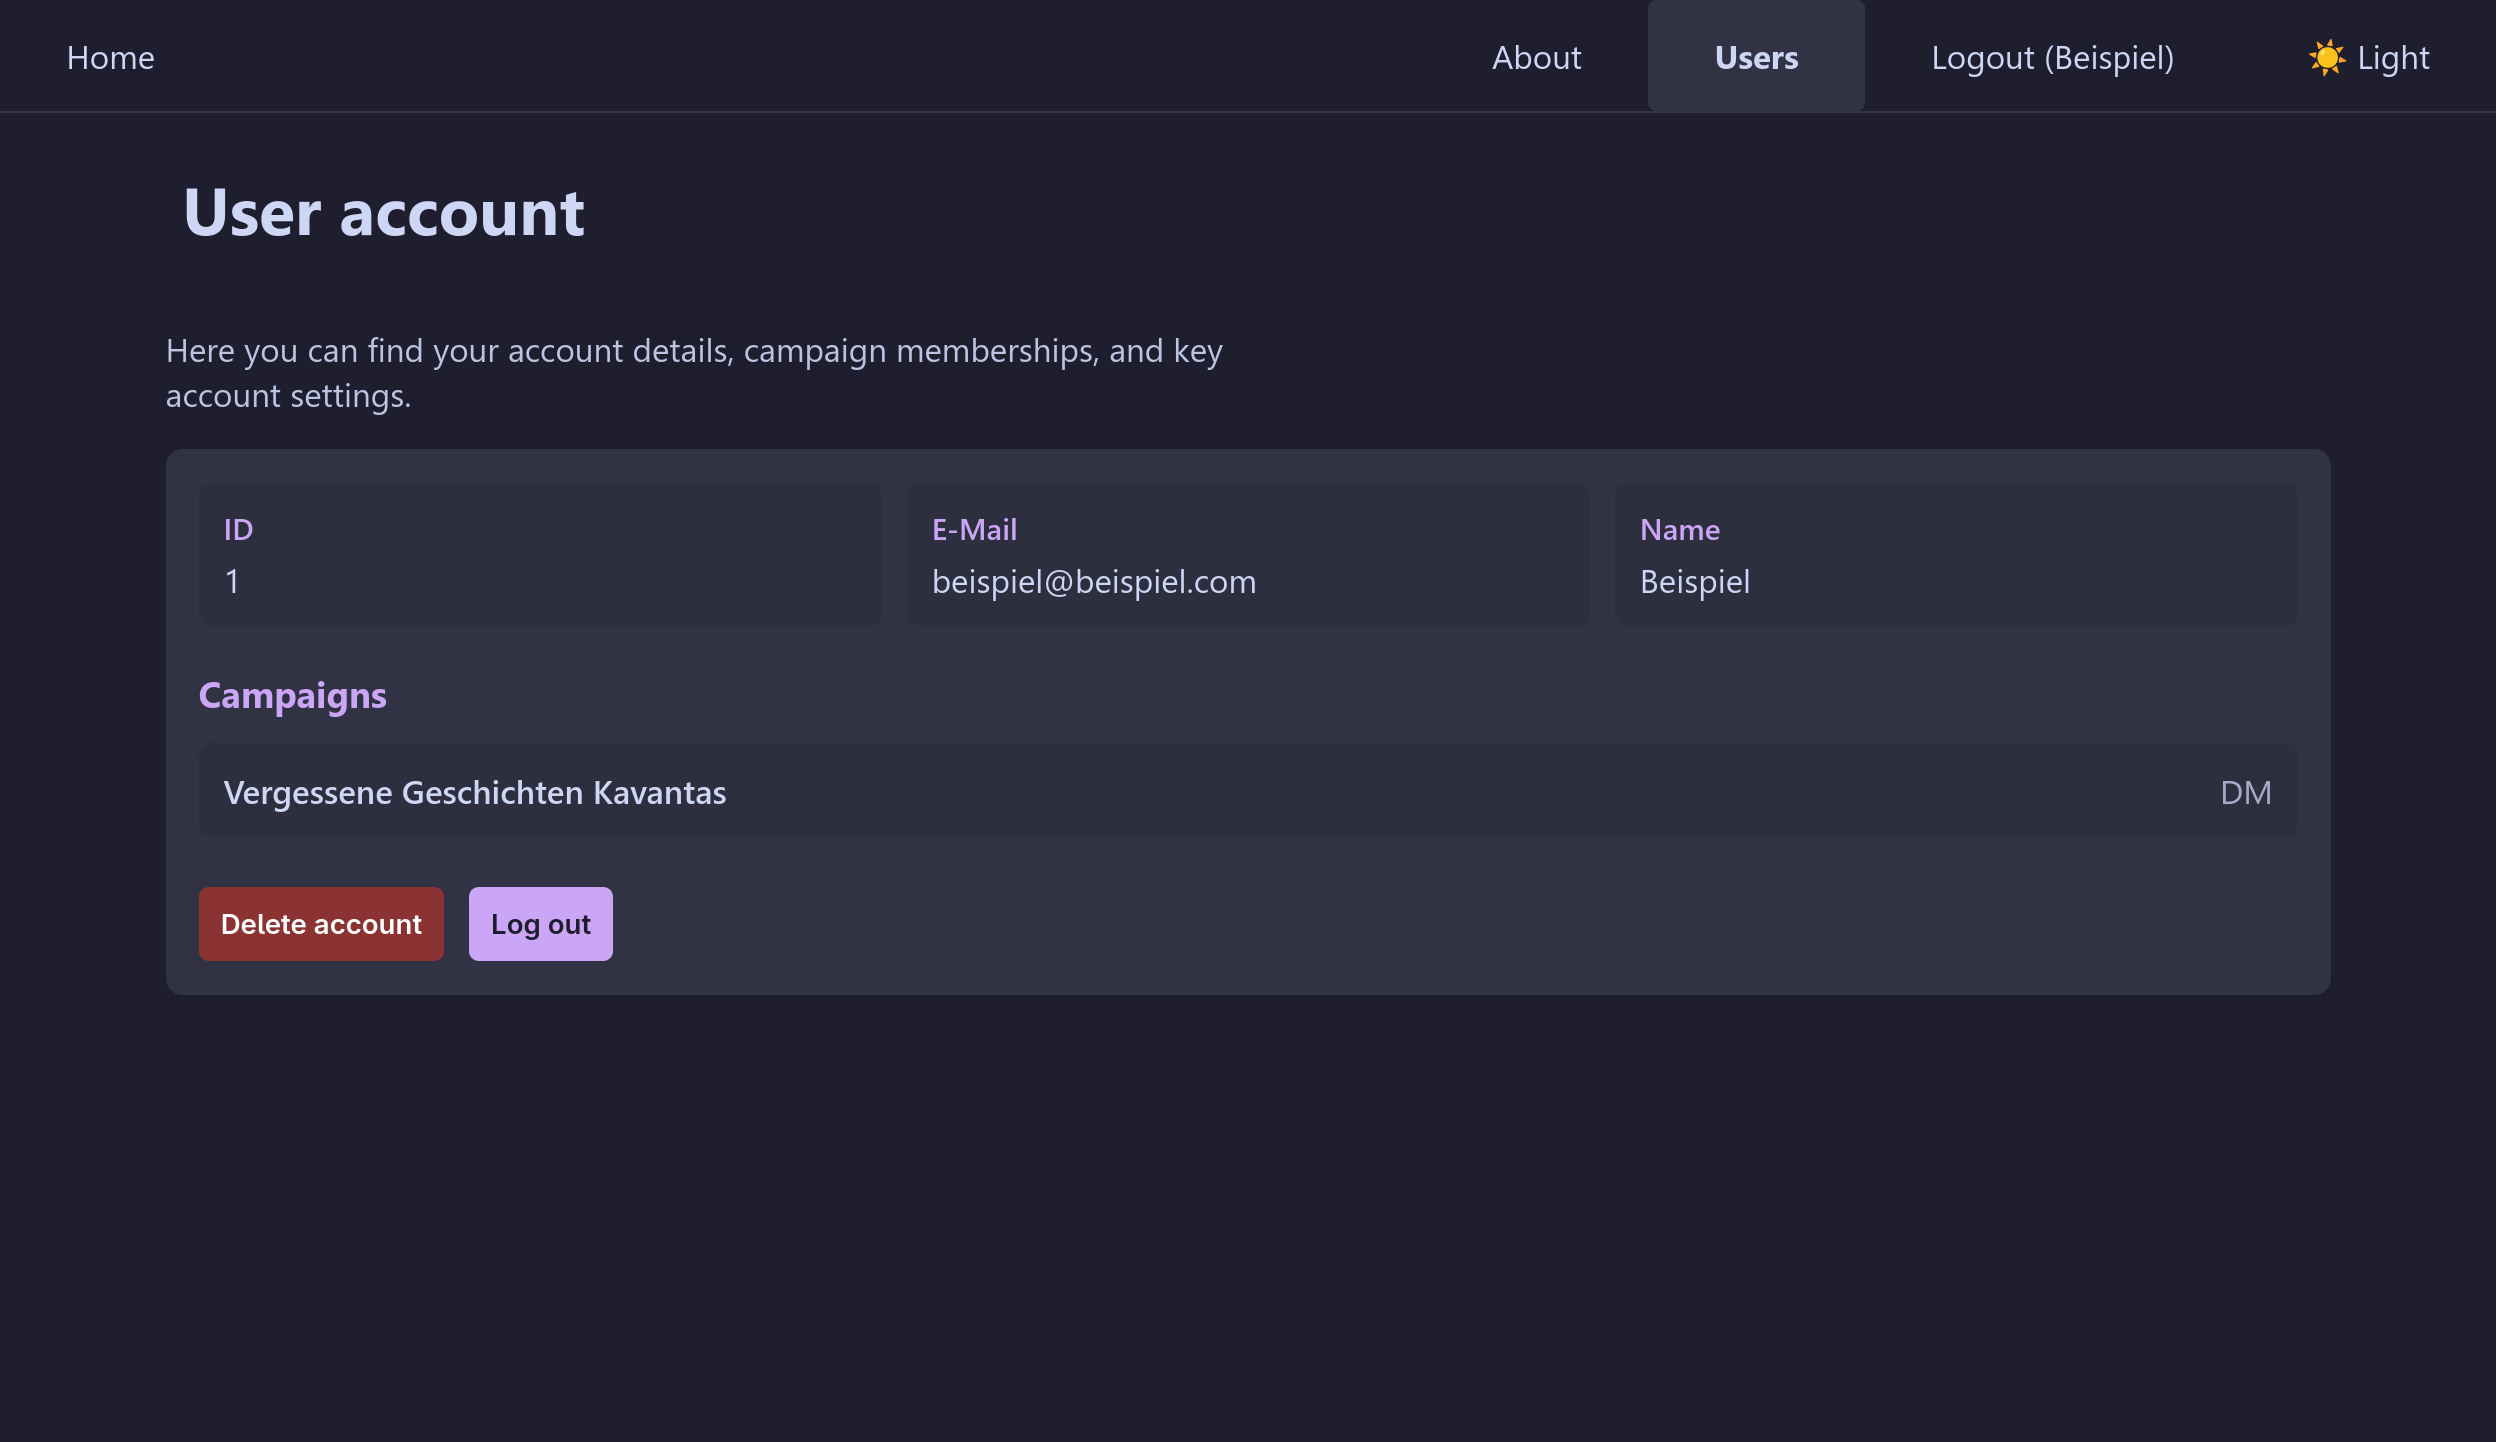
\includegraphics[width=0.92\textwidth]{media/Users.png}
  \caption{User-/Mitgliederansicht}
\end{figure}

\section{Formales und Quellenhinweise}

\subsection{Formale Anforderungen}
\begin{itemize}
  \item Ausgabe als PDF mit sauberem Layout.
  \item Deckblatt mit Namen, Matrikelnummern, Projekttitel und Abgabedatum.
  \item Quellenangaben bei maßgeblich genutzten externen Ressourcen.
\end{itemize}

\subsection{Quellen}
Alle externen Quellen werden im Literaturverzeichnis und bei Bedarf direkt im Fließtext referenziert.


% --- Literaturverzeichnis ---
\newpage
\printbibliography[heading=bibintoc, title={Literaturverzeichnis}]
\end{document}
